\section{Čas izumrtja populacije}
Z diferencialno enačbo
\begin{equation}
    \dot N = -\beta\,N
\end{equation}
in začetnimi pogoji je podan sistem za izumiranje populacije, ki se na stohastičen način popiše
\begin{equation}
    N_{i+1} = N_i -\mathcal{P}(\beta\,N_i\,\Delta t)
\end{equation}
kjer je $\mathcal{P}(\lambda)$ naključno število iz Poissonske porazdelitve okoli srednje vrednost $\lambda$, prikazane na spodnji sliki. Faktor $\beta$ podaja hitrost upadanja.

\begin{figure}[ht]
    \centering
    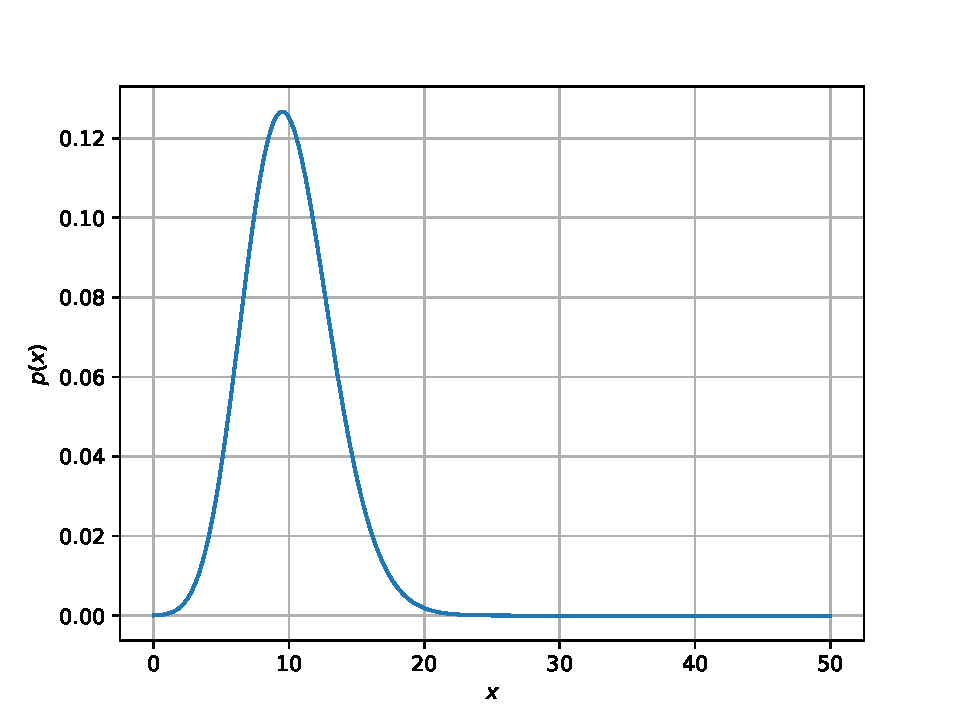
\includegraphics[width=0.5\linewidth]{9.nal_slike/poisson.pdf}
    \caption{Poissonska porazdelitev okoli sr. vrednosti $\lambda=10$}
\end{figure}

Na spodnji sliki je prikazan potek populacije in primerjava med stohastičnim in analitičnim modelom ter numerično integracijo v času. Zaradi naključnosti v generiranju števil potek stohastičnega modela variira od ponovitev in okoli analitične krivulje, saj lahko zavzema le cela števila. Prav tako pa z večanjem populacije odstopanje postaja vedno manjše. V takem primeru je analitična rešitev oblike $N(t) = N_0 \, e^{\beta\,t}$.

\begin{figure}[H]
    \centering
    \begin{subfigure}{\textwidth}
        \centering
        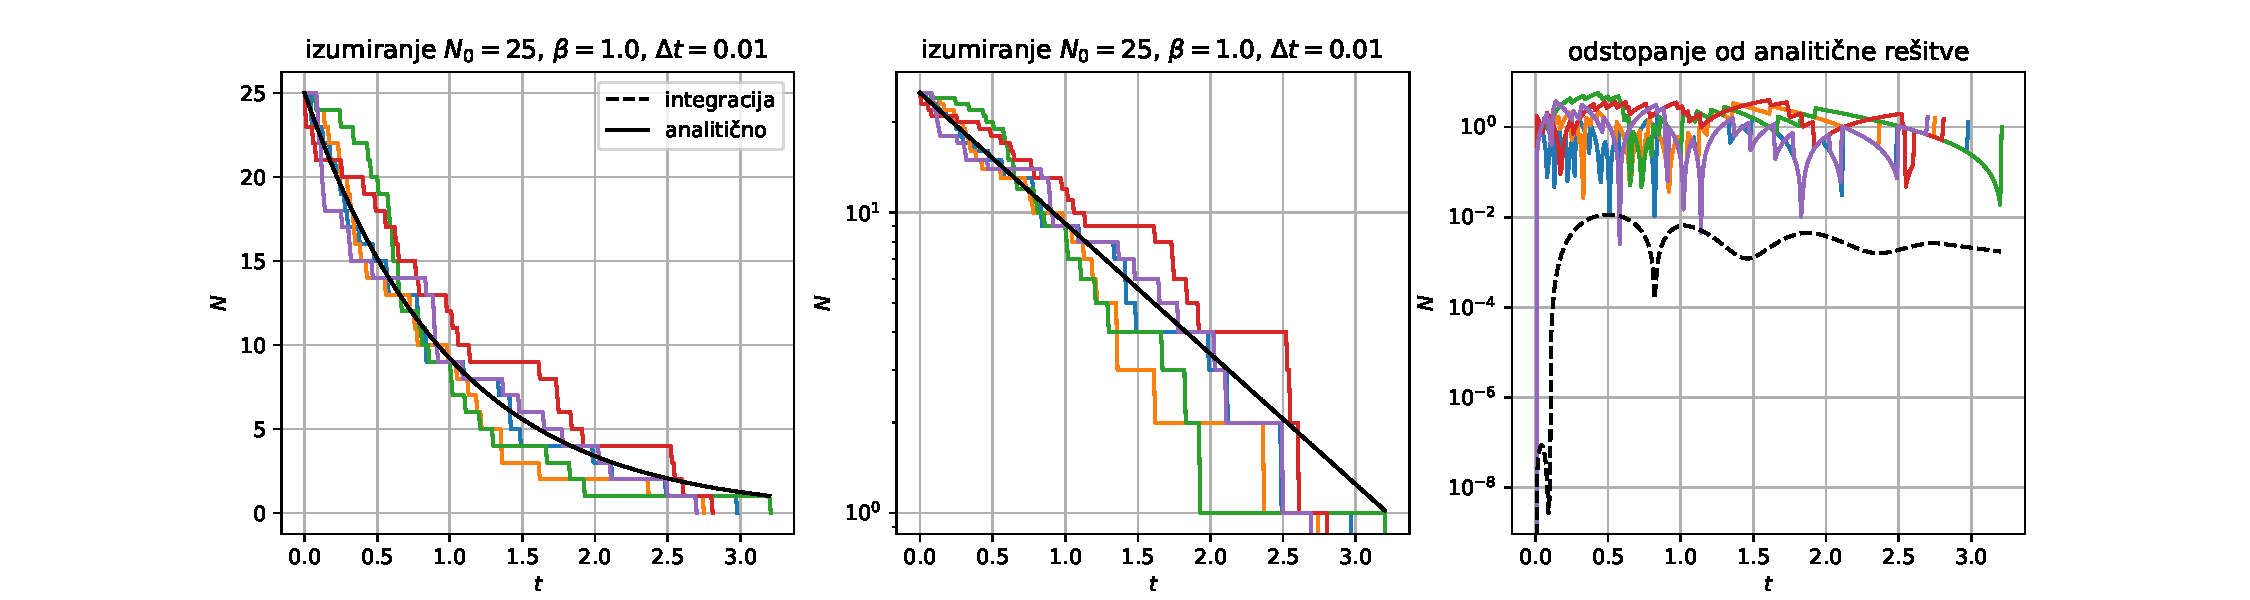
\includegraphics[width=\linewidth]{9.nal_slike/1/izumiranje_N025.pdf}
        \caption{$N_0=25$}
    \end{subfigure}
    \begin{subfigure}{\textwidth}
        \centering
        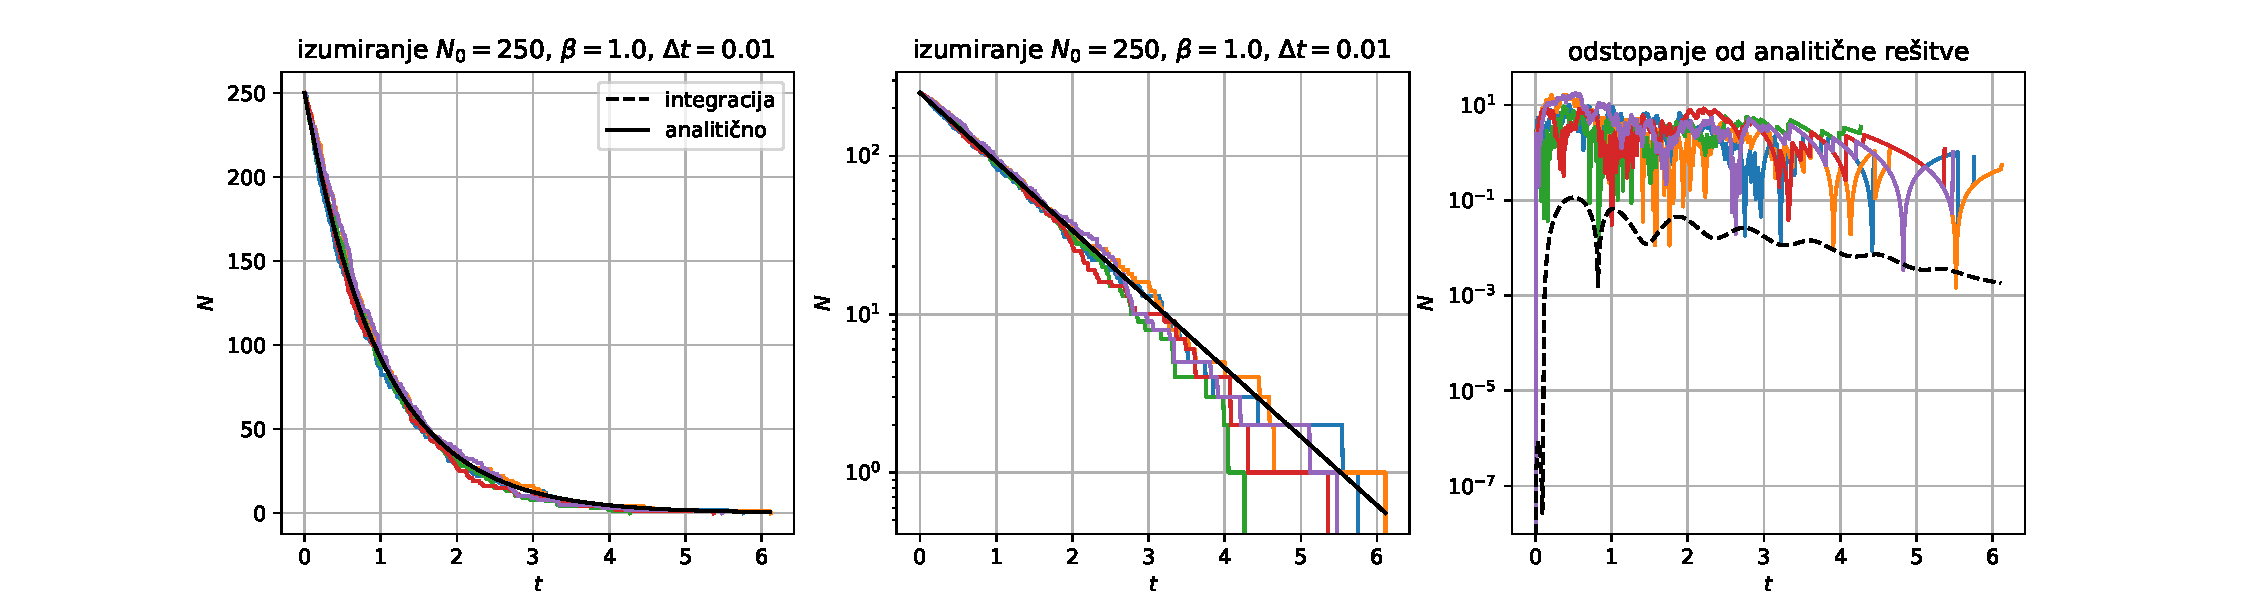
\includegraphics[width=\linewidth]{9.nal_slike/1/izumiranje_N0250.pdf}
        \caption{$N_0=250$}
    \end{subfigure}
    \caption{Izumiranje populacije z $\beta=1$}
\end{figure}

Pri stohastičnem modelu lahko spremljamo tudi čas izumrtja, dočim pri preostalih zaradi zvezne narave in eksponentne ga upada to ni popolnoma mogoče. Na spodnji sliki so prikazane porazdelitve časov izumrtja za različne koeficiente $\beta$ in velikosti populacije.

\begin{figure}[ht]
    \centering
    \begin{subfigure}{0.49\textwidth}
        \centering
        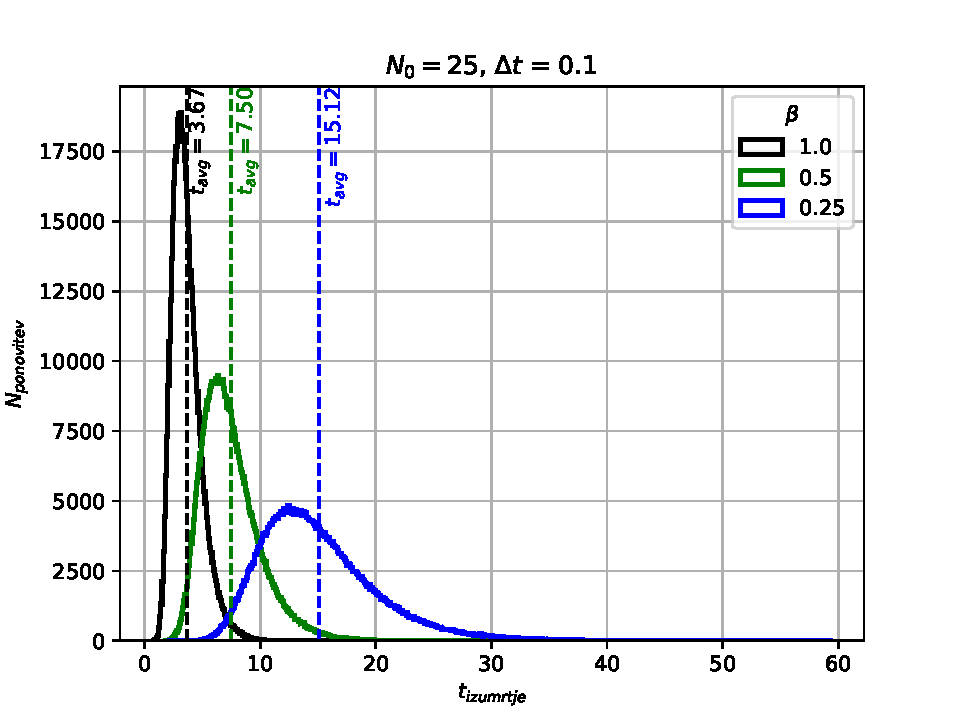
\includegraphics[width=\linewidth]{9.nal_slike/1/t_izumrtja_N025.pdf}
        \caption{$N_0=25$}
    \end{subfigure}
    \begin{subfigure}{0.49\textwidth}
        \centering
        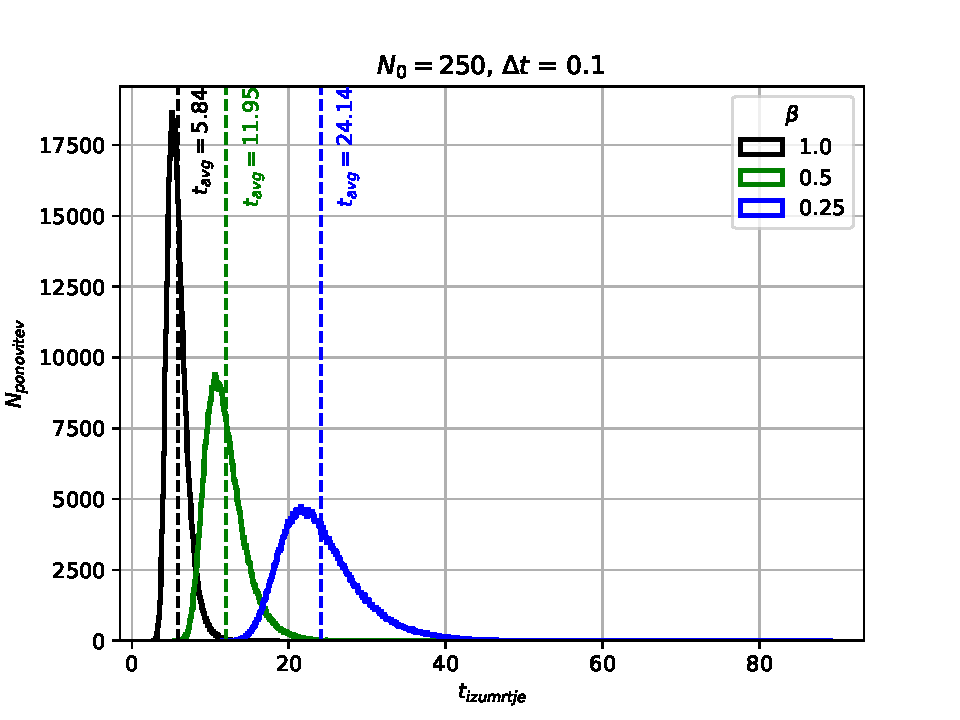
\includegraphics[width=\linewidth]{9.nal_slike/1/t_izumrtja_N0250.pdf}
        \caption{$N_0=250$}
    \end{subfigure}
    \caption{Porazdelitev časov izumrtja, 500 000 ponovitev}
\end{figure}

Če upoštevamo še rojstva in smrti, se modelu za izumiranje populacije doda nov člen:
\begin{equation}
    N_{i+1} = N_i -\mathcal{P}(\beta_s\,N_i\,\Delta t) +\mathcal{P}(\beta_r\,N_i\,\Delta t)
\end{equation}
kjer sta $\beta_s$ in $\beta_r$ faktorja za smrti in rojstva.

\begin{figure}[H]
    \centering
    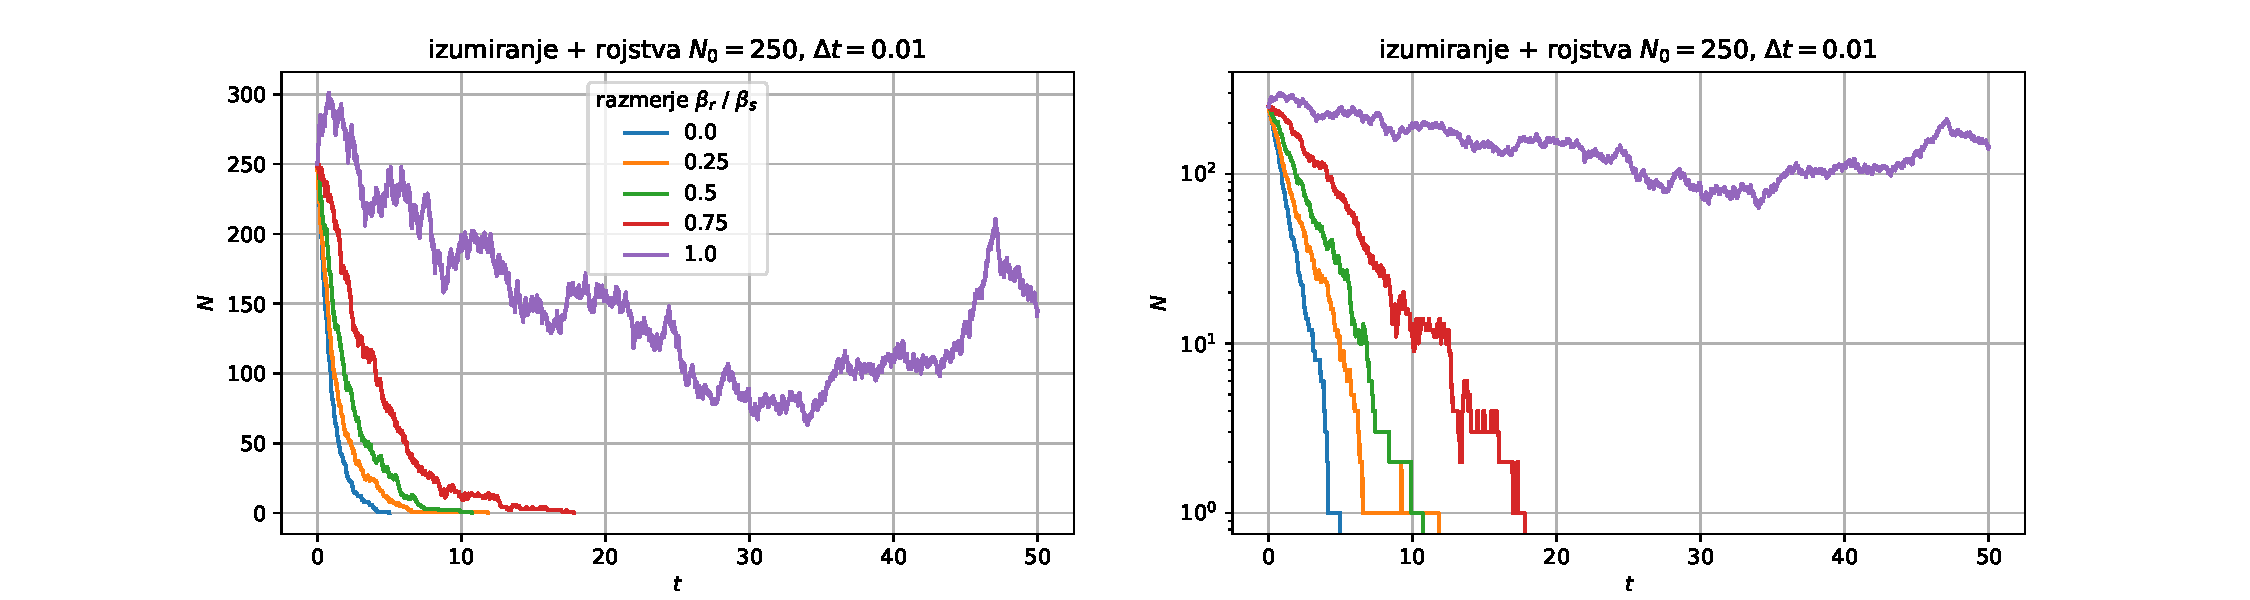
\includegraphics[width=\linewidth]{9.nal_slike/1/izumiranje_rojstva_N0250.pdf}
    \caption{Izumiranje populacije z upoštevanjem rojstev}
\end{figure}

Kot smo videli, z naključnim modelom ne dobimo vedno enake vrednosti časa izumrtja, zato sem prikazal kako je odvisen povprečen čas izumrtja populacije 10 000 simulacij od parametrov, kar je prikazano na spodnjih dveh slikaz za oba modela.

\begin{figure}[H]
    \centering
    \begin{subfigure}{0.49\textwidth}
        \centering
        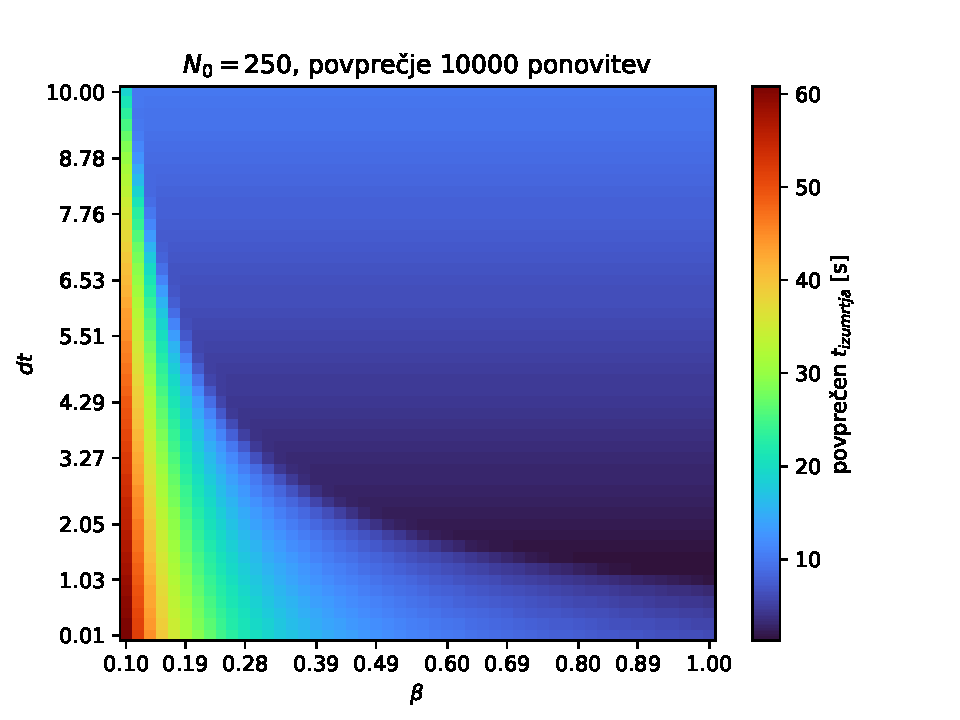
\includegraphics[width=\linewidth]{9.nal_slike/1/izumrtje_dt_beta_le_smrti.pdf}
        \caption{brez rojstev}
    \end{subfigure}
    \begin{subfigure}{0.49\textwidth}
            \centering
        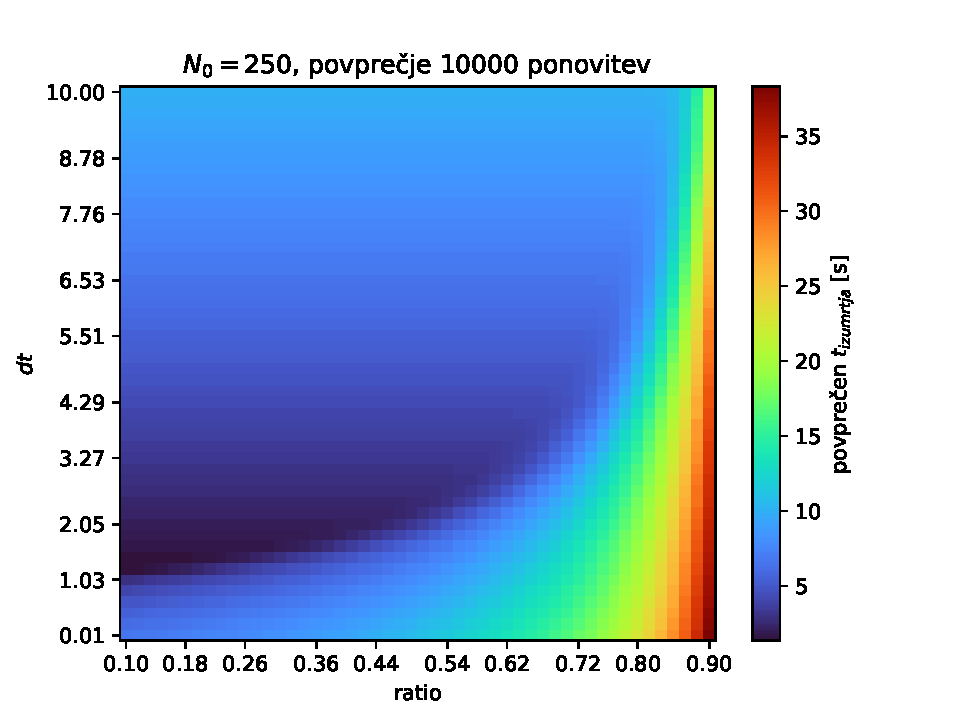
\includegraphics[width=\linewidth]{9.nal_slike/1/izumrtje_dt_ratio.pdf}
        \caption{z rojstvi}
    \end{subfigure}
    \caption{Vpliv parametrov ($\Delta t$, $\beta$, $ratio$) na čas izumrtja}
\end{figure}

Na spodnji sliki sem prikazal s kakšno verjetnostjo je ob nekem času določeno število osebkov. Opazim, da vključitev rojstev rezširi območje raztrosa. Pri $ratio=1$ bi sicer pričakoval vodoravno črto.

\begin{figure}[H]
    \centering
    \begin{subfigure}{0.49\textwidth}
        \centering
        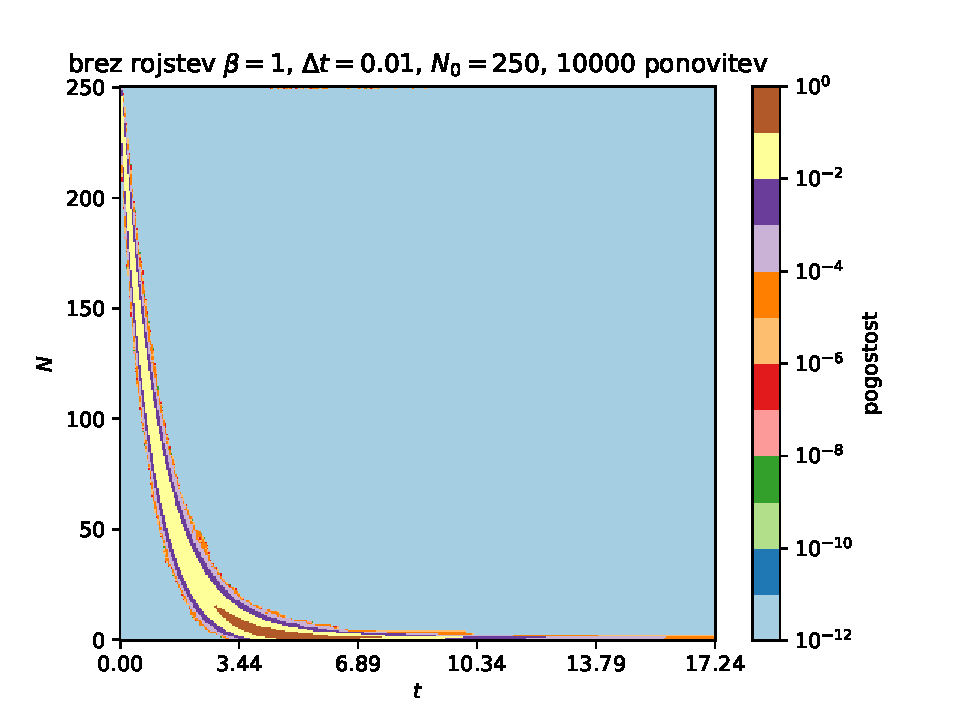
\includegraphics[width=\linewidth]{9.nal_slike/1/verjetnost_poteka_ratio0.0.pdf}
        \caption{ratio = 0}
    \end{subfigure}
    \begin{subfigure}{0.49\textwidth}
            \centering
        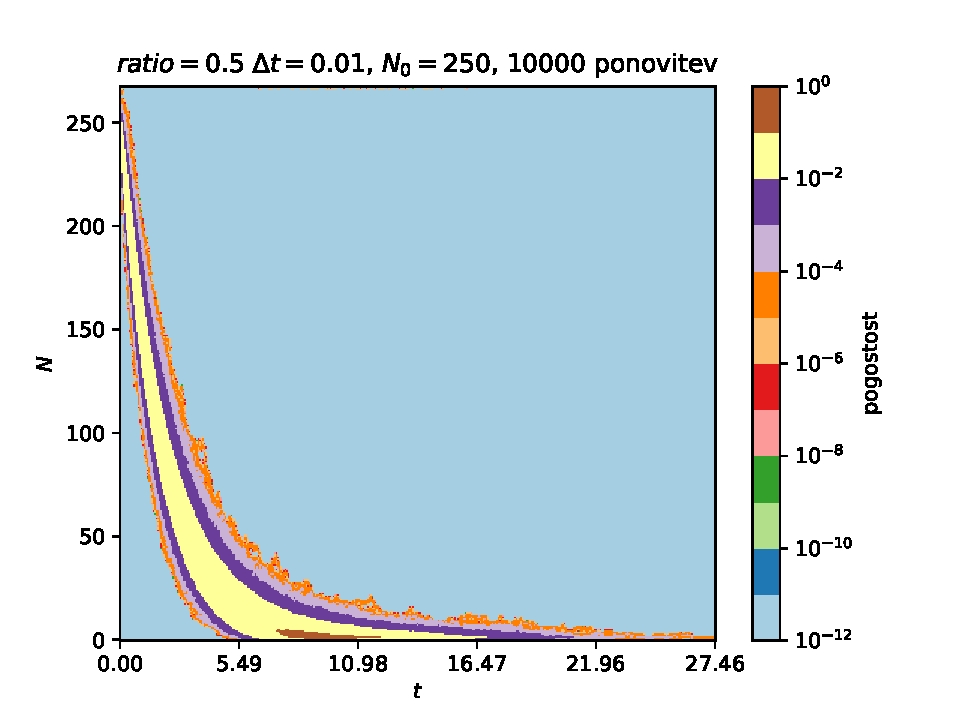
\includegraphics[width=\linewidth]{9.nal_slike/1/verjetnost_poteka_ratio0.5.pdf}
        \caption{ratio = 0,5}
    \end{subfigure}
    \caption{Verjetnost poteka izumiranja glede na pogostost potekov 10 000 ponovitev (1/2)}
\end{figure}

\begin{figure}[H]
    \centering
    \begin{subfigure}{0.49\textwidth}
        \centering
        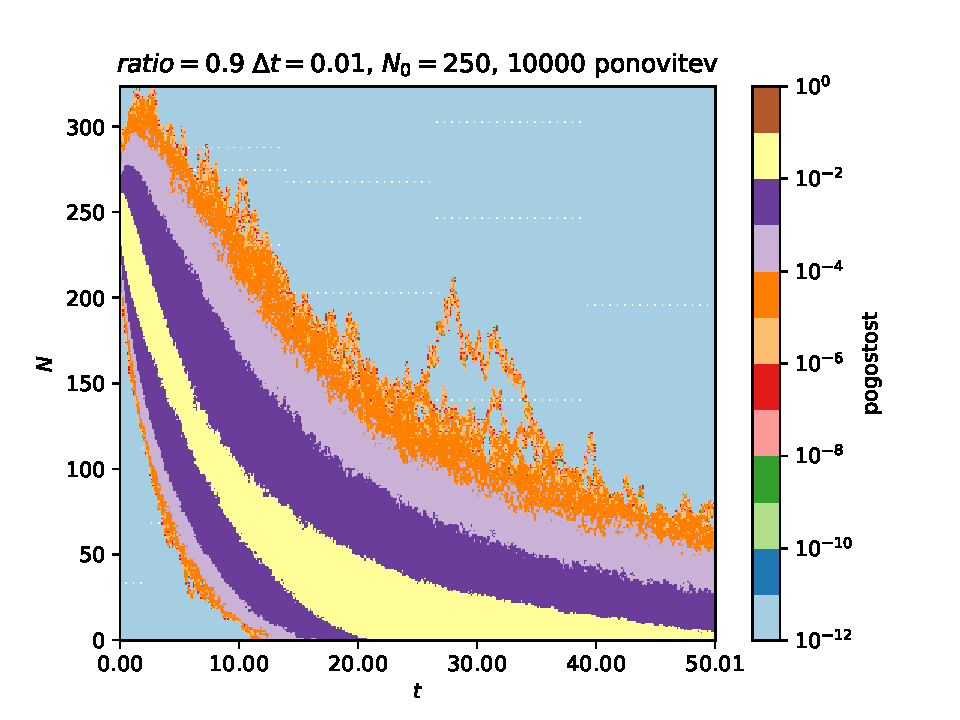
\includegraphics[width=\linewidth]{9.nal_slike/1/verjetnost_poteka_ratio0.9.pdf}
        \caption{ratio = 0,9}
    \end{subfigure}
    \begin{subfigure}{0.49\textwidth}
            \centering
        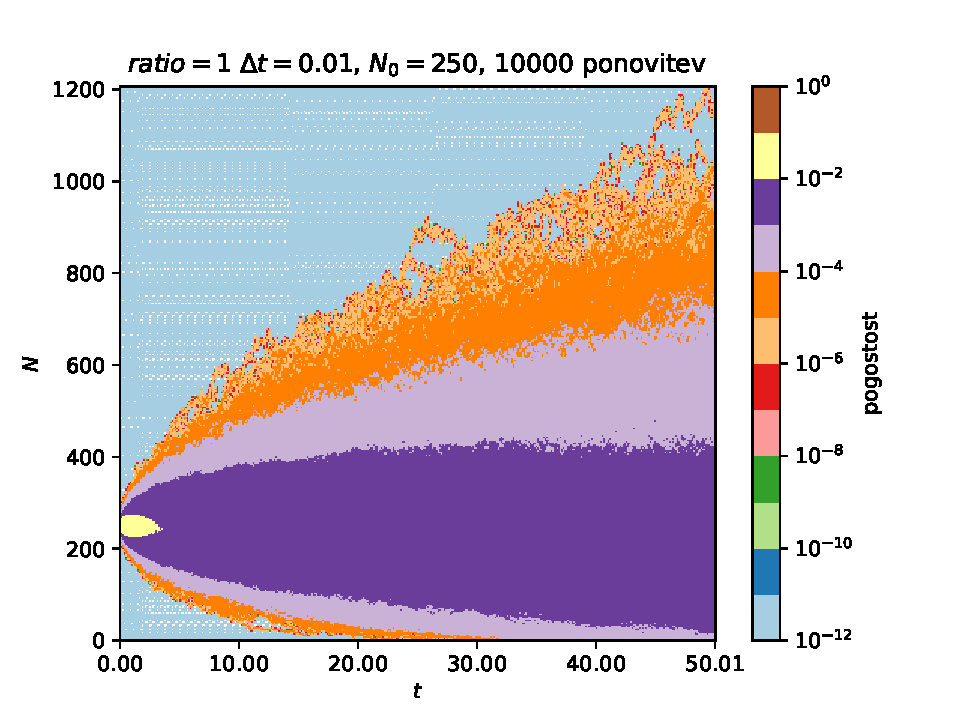
\includegraphics[width=\linewidth]{9.nal_slike/1/verjetnost_poteka_ratio1.pdf}
        \caption{ratio = 1}
    \end{subfigure}
    \caption{Verjetnost poteka izumiranja glede na pogostost potekov 10 000 ponovitev (2/2)}
\end{figure}

\section{Matrična formulacija}

Sistem lahko rešujemo tudi drugače; s pomočjo statistike, namesto z generiranjem naključnih števil. Pri tem razdelimo velikost populacije na $N$ diskretnih nivojev, ki se opiše z vektorjem stanja sistema $x(t)$. S pomočjo matrike prehodov, ki se izpelje iz verjetnostne porazdelitve, lahko izračunamo prihodje stanje
\begin{equation}
    \mathbf{x}(t+\Delta t) = M \cdot \mathbf{x}(t),
\end{equation}
kjer je $M$ matrika prehodov, ki je tridiagonalna.
\begin{align}
    M_{i,i-1} &= R_{i-1}\,\Delta t\\ \nonumber
    M_{i,i} &= 1-\Delta t\, (R_{i}+S_i)\\ \nonumber
    M_{i,i+1} &= S_{i+1}\,\Delta t,
\end{align}
kjer je $R_i=i\,\beta_r$ in $S_i=i\,\beta_s$. Pri tem velja pravilo, da mora biti vsota vsakega stolpca enaka ena, kar zadovolji zahtevo po ohranitvi populacije preko nivojev. 

\begin{figure}[ht]
    \centering
    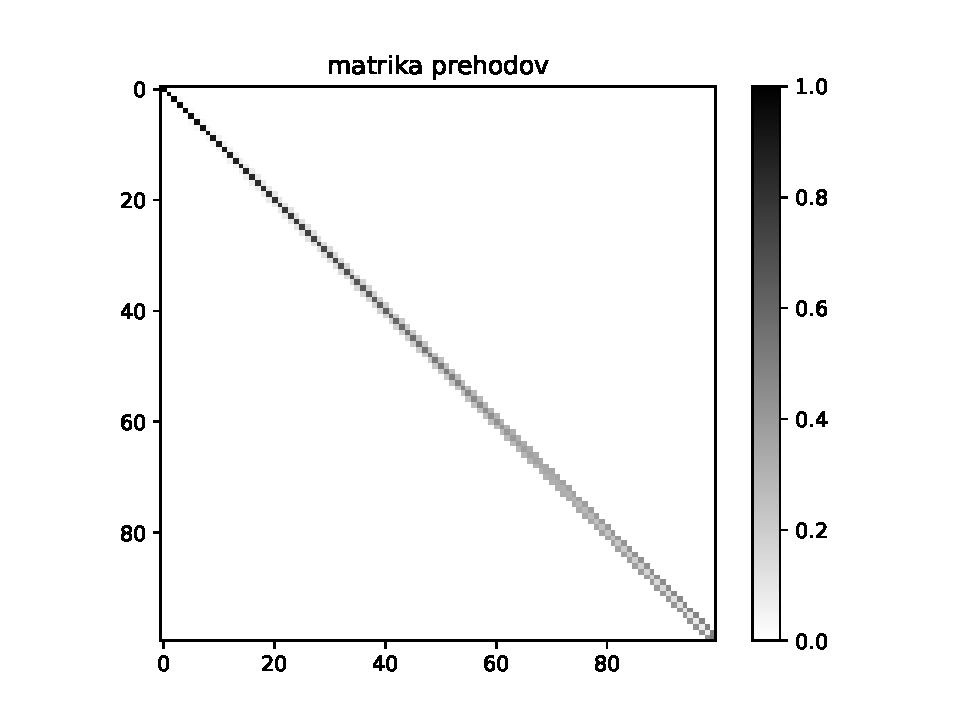
\includegraphics[width=0.7\linewidth]{9.nal_slike/2/matrika_prehodov.pdf}
    \caption{Matrika prehodov za stabilen sistem je diagonalno dominatna}
\end{figure}

%GIF ANIMACIJE !!!!!!!!!!!!!!!!!!
% \includemovie{0.5\textwidth}{0.5\textwidth}{9.nal_slike/2/nivoji10_ratio0.0.gif}

Kot začetni pogoj sem predpisal, da je v najvišjem nivoju celotna populacija (100\%) in nato iteriral, dokler ni bilo v najnižjem nivoju vsaj 99\% celotne populacije. V spodnjih \textit{gif} slikah je moč videti, kako je porazdeljena verjetnost za populacijo na nekem nivoju ob nekem času oz. kako eksponentno izumirajo osebki. Presenetljivo je, da večanje rojstev (večji $ratio$) pomeni hkrati z večjim časom izumrtja tudi večji raztros verjetnostne porazdelitve po nivojih, kar je opazno tudi na slikah s statističnimi velikinami, izračunanimi po enačbi za i-ti statistični moment
\begin{equation}
    \mu_i(t) = \frac{1}{\sigma^i}\;\sum_{n=0}^{N}\;n^i\,x_n(t),
\end{equation}
kjer je $\sigma$ standardni odklon in $x_n$ stanje v n-tem nivoju.
Povprečno vrednost sem računal po enačbi
\begin{equation}
    \mu(t) = X_0\, e^{-(\beta_r-\beta_s)\,t}.
\end{equation}

\begin{figure}[H]
    \centering
    \begin{subfigure}{0.49\textwidth}
        \centering
        \href{run:./animacije/nivoji10_ratio0.0.gif}{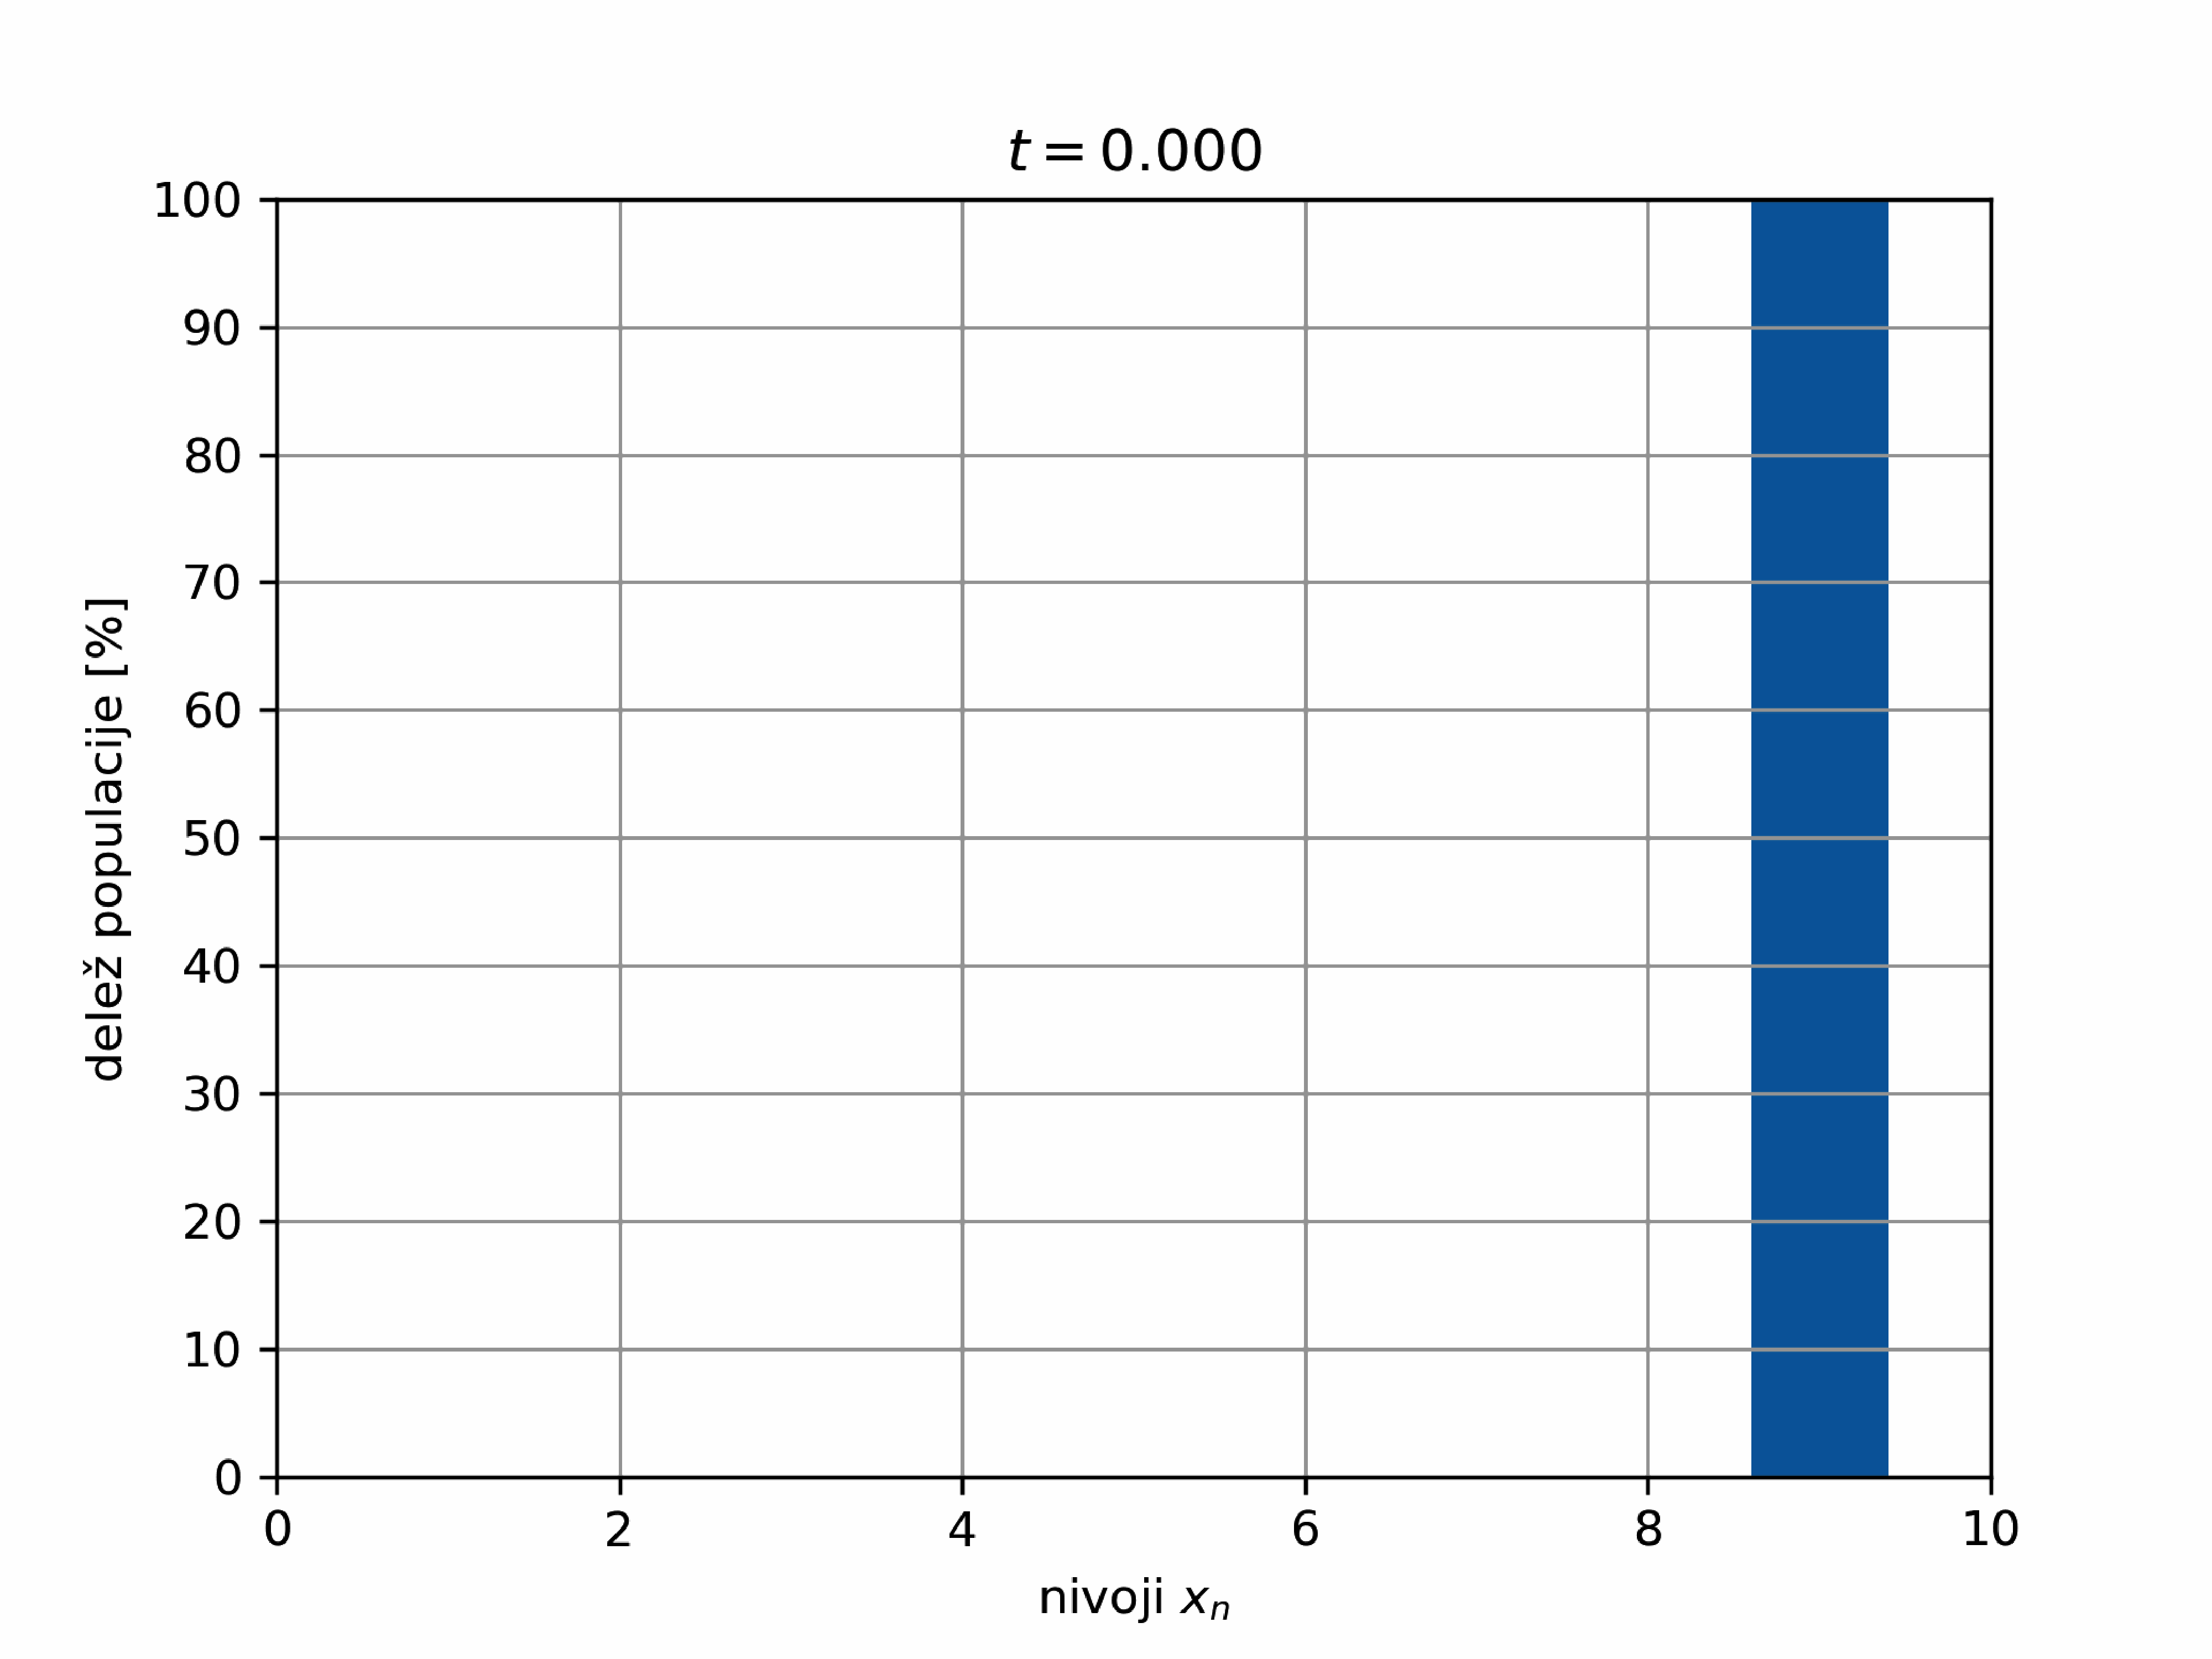
\includegraphics[width=0.5\textwidth]{9.nal_slike/2/nivoji10_ratio0.0.pdf}} %./podmapa, ../pod-podmapa
        \caption{nivoji10\_ratio0.0}
    \end{subfigure}
    \begin{subfigure}{0.49\textwidth}
        \centering
        \href{run:./animacije/nivoji10_ratio0.0.gif}{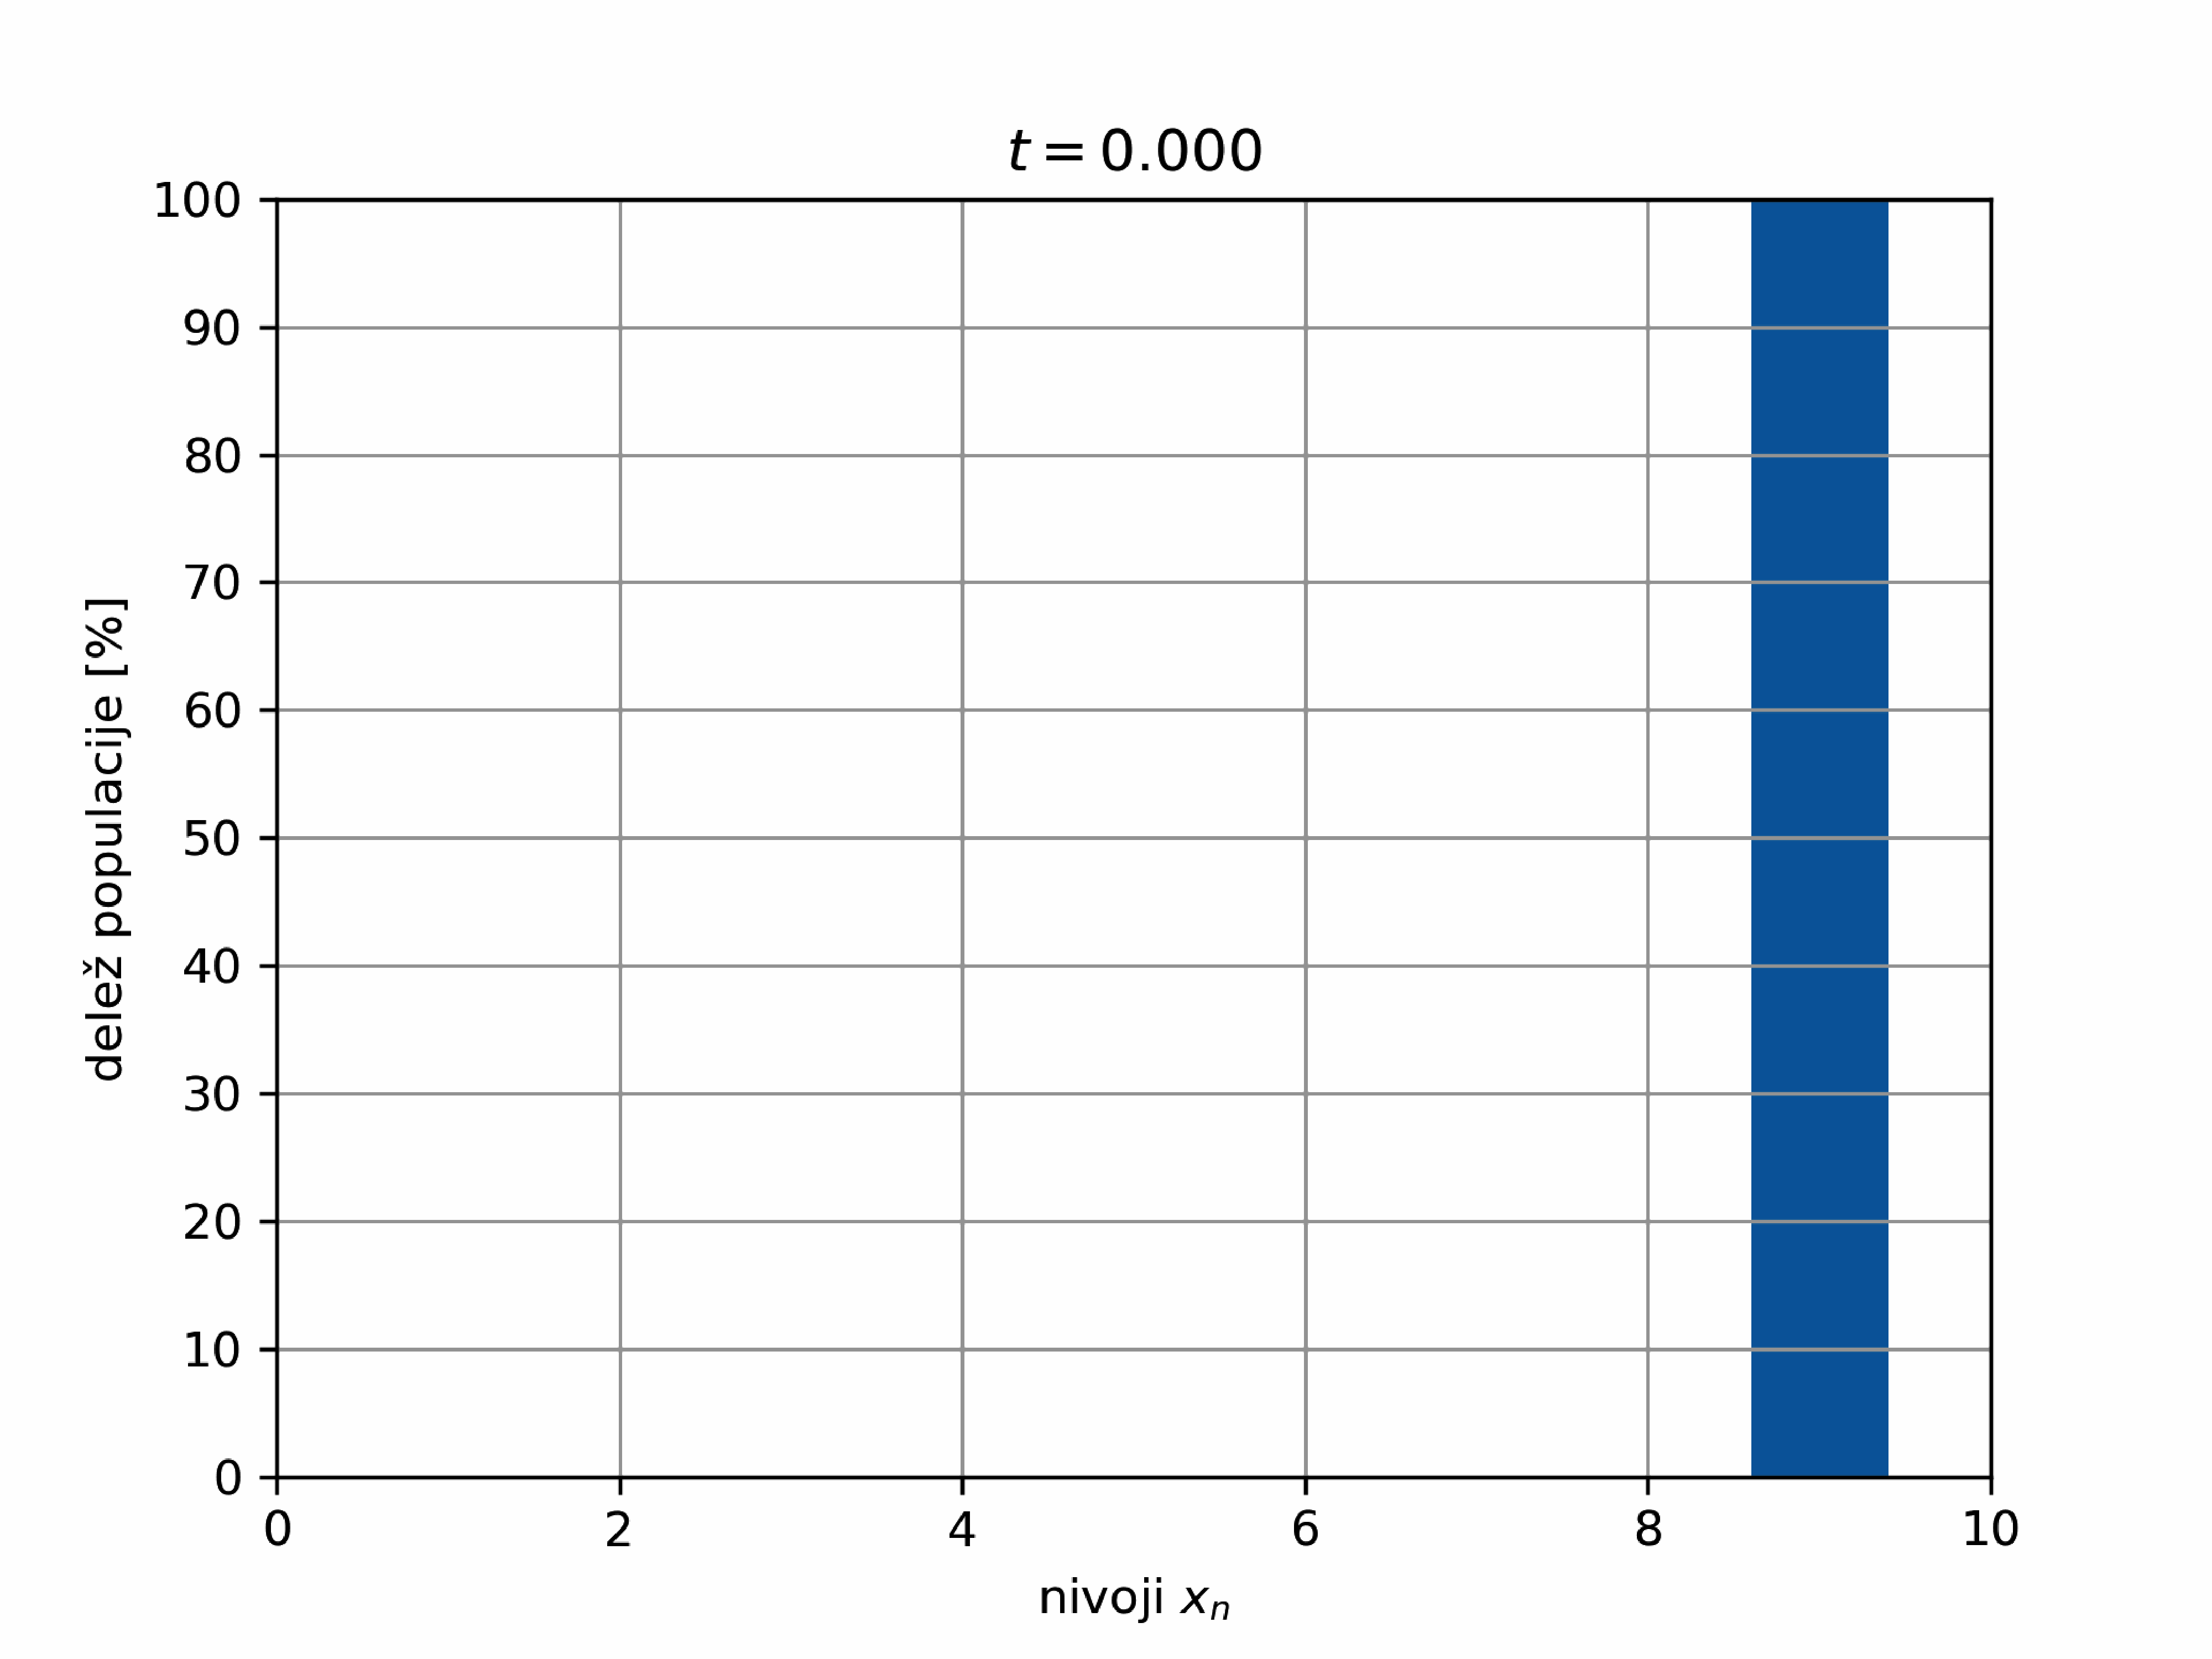
\includegraphics[width=0.5\textwidth]{9.nal_slike/2/nivoji10_ratio0.9.pdf}}
        \caption{nivoji100\_ratio0.9}
    \end{subfigure}
    \caption{Za prikaz simulacije kliknite, datoteke so shranjene v podmapi \textit{animacije}.}
\end{figure}

\begin{figure}[H]
    \centering
    \begin{subfigure}{0.49\textwidth}
        \centering
        \href{run:./animacije/nivoji10_ratio0.0.gif}{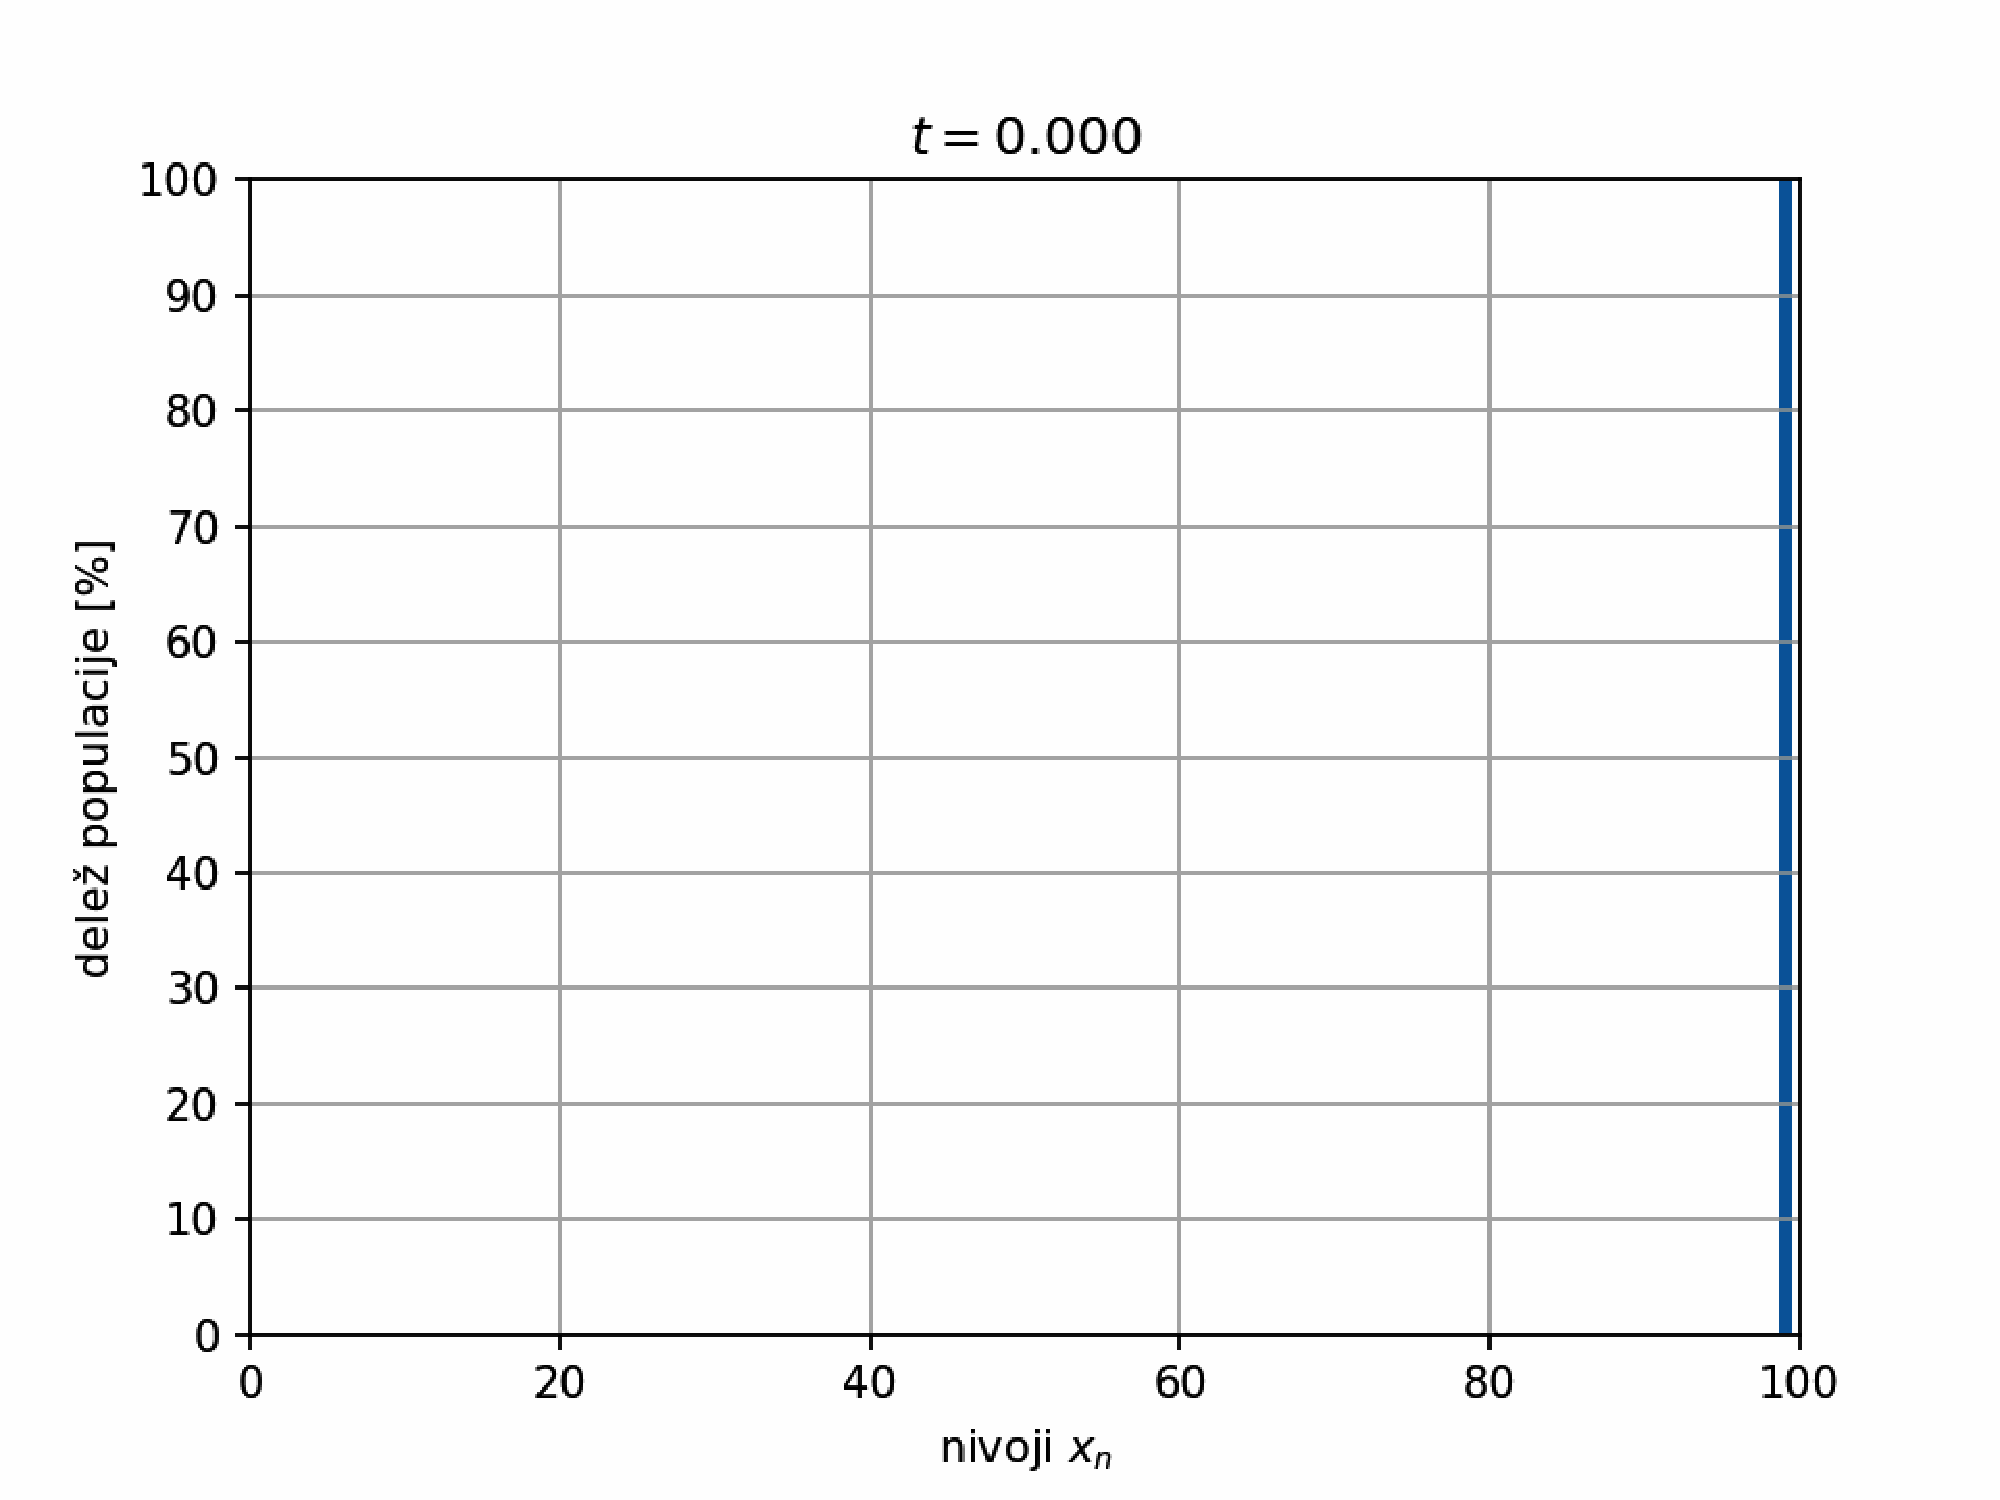
\includegraphics[width=0.5\textwidth]{9.nal_slike/2/nivoji100_ratio0.0.pdf}}
        \caption{nivoji100\_ratio0.0}
    \end{subfigure}
    \begin{subfigure}{0.49\textwidth}
        \centering
        \href{run:./animacije/nivoji10_ratio0.0.gif}{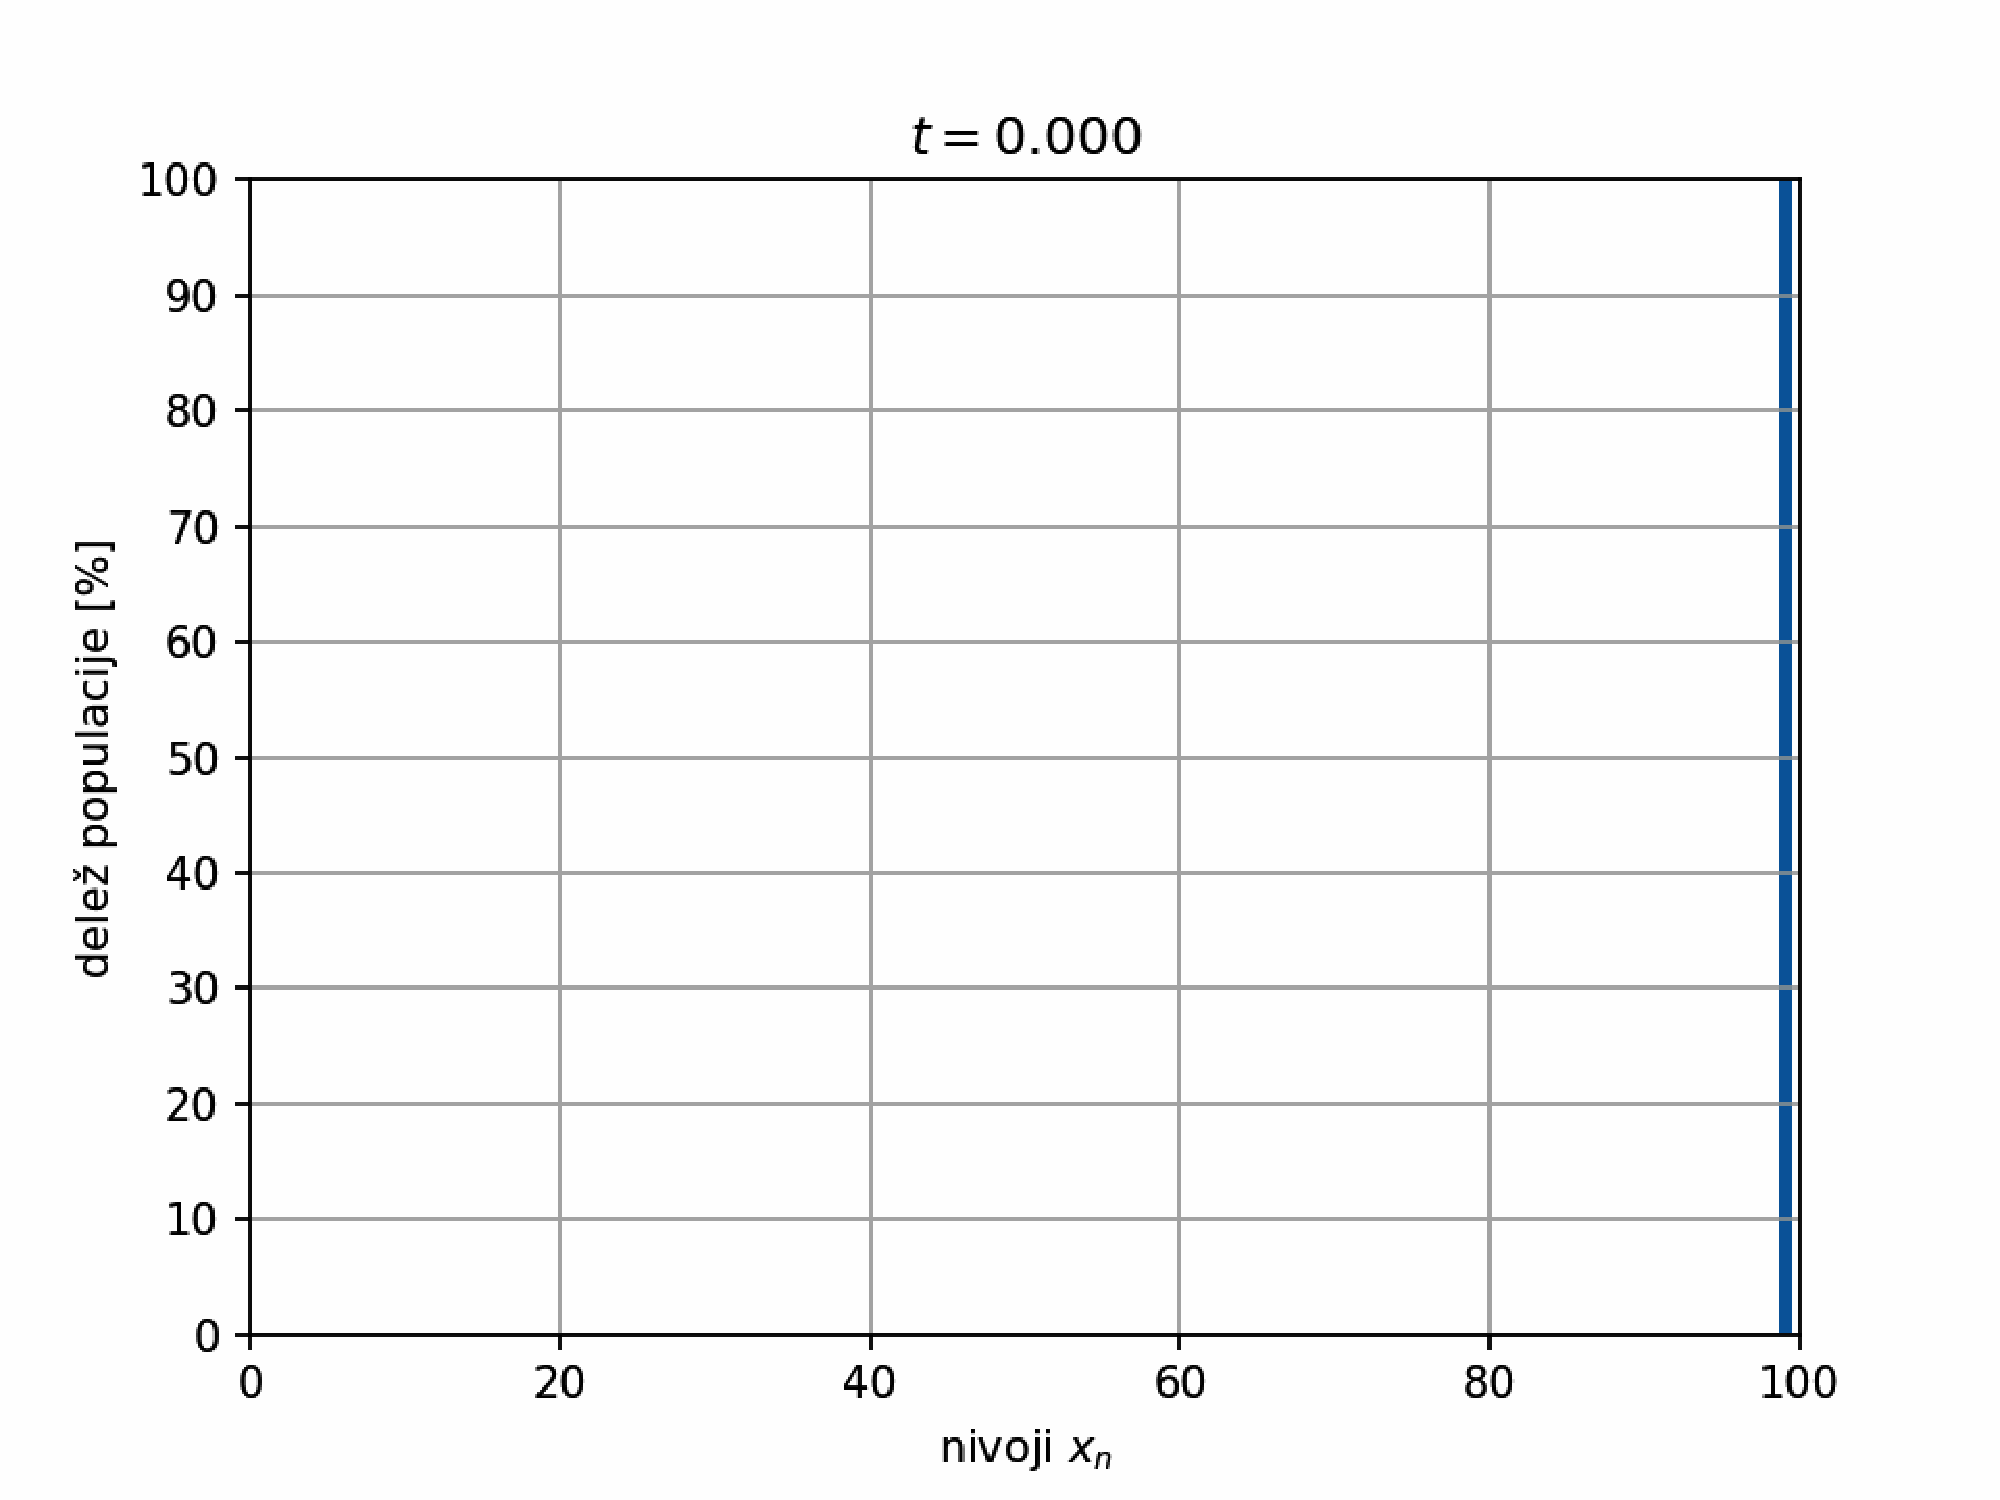
\includegraphics[width=0.5\textwidth]{9.nal_slike/2/nivoji100_ratio0.9.pdf}}
        \caption{nivoji100\_ratio0.9}
    \end{subfigure}
    \caption{Za prikaz simulacije kliknite, datoteke so shranjene v podmapi \textit{animacije}.}
\end{figure}

\begin{figure}[ht]
    \centering
    \begin{subfigure}{0.49\textwidth}
        \centering
        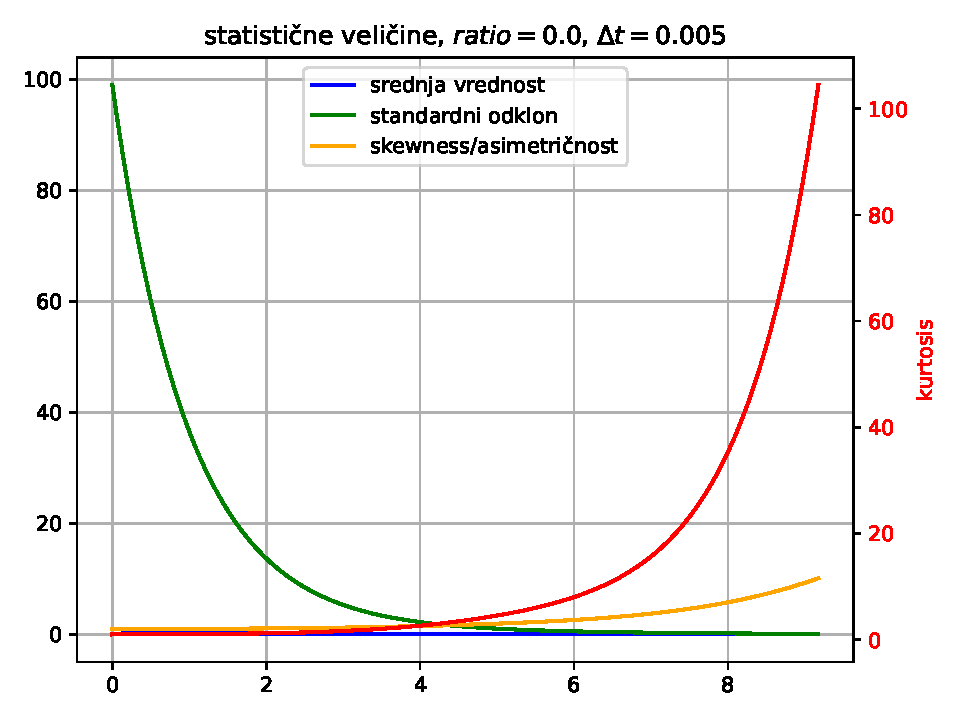
\includegraphics[width=\linewidth]{9.nal_slike/2/stat_vel_ratio0.0.pdf}
        \caption{ratio = 0, $\beta=1$}
    \end{subfigure}
    \begin{subfigure}{0.49\textwidth}
        \centering
        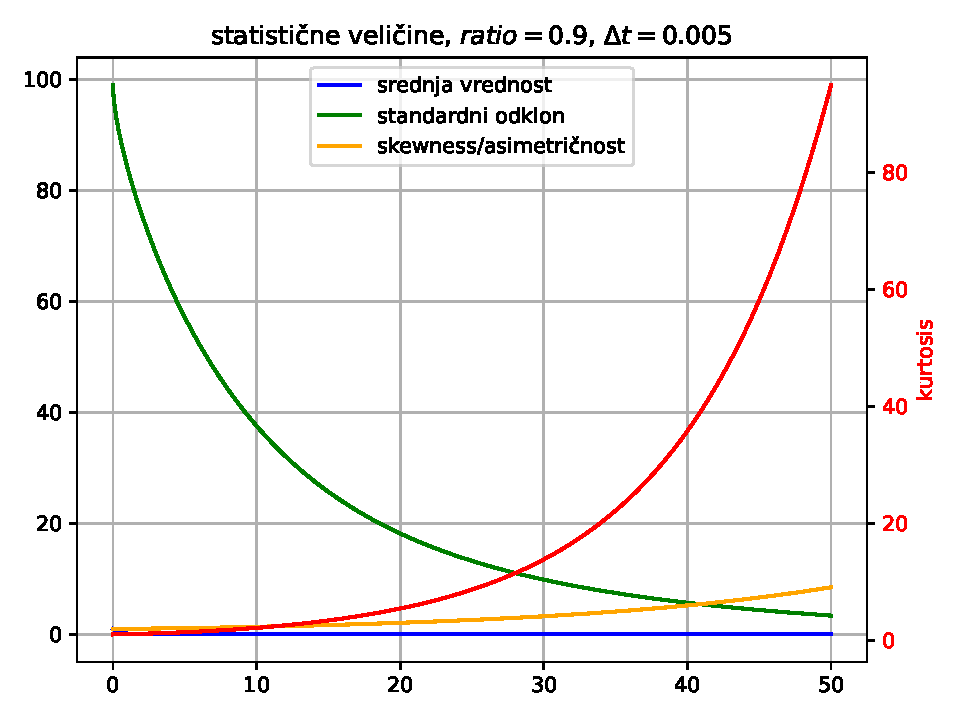
\includegraphics[width=\linewidth]{9.nal_slike/2/stat_vel_ratio0.9.pdf}
        \caption{ratio=0,9}
    \end{subfigure}
    \caption{Potek statistčnih veličin}
\end{figure}

Iz primerjavo s prejšnjo (naključno) metodo sem ugotovil, da se statistična bolje prilega analitični rešitvi, sploh pri nižjem $ratio$. Pri višjem je odstopanje vedno večje, pri primerjevi časa izumrtja pa razlika med modeloma narašča z večanjem $ratio$. Mogoče bi bilo potrebno v povprečje zajeti več poskusov.

\begin{figure}[ht]
    \centering
    \begin{subfigure}{0.49\textwidth}
        \centering
        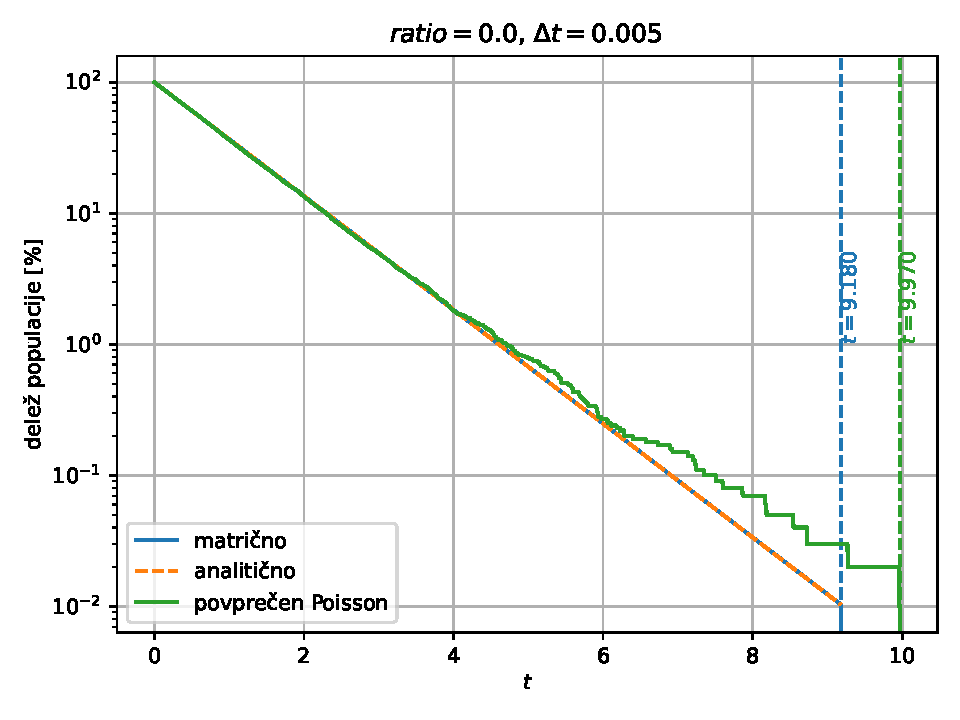
\includegraphics[width=\linewidth]{9.nal_slike/2/primerjava_ratio0.0.pdf}
        \caption{ratio = 0, $\beta=1$}
    \end{subfigure}
    \begin{subfigure}{0.49\textwidth}
            \centering
        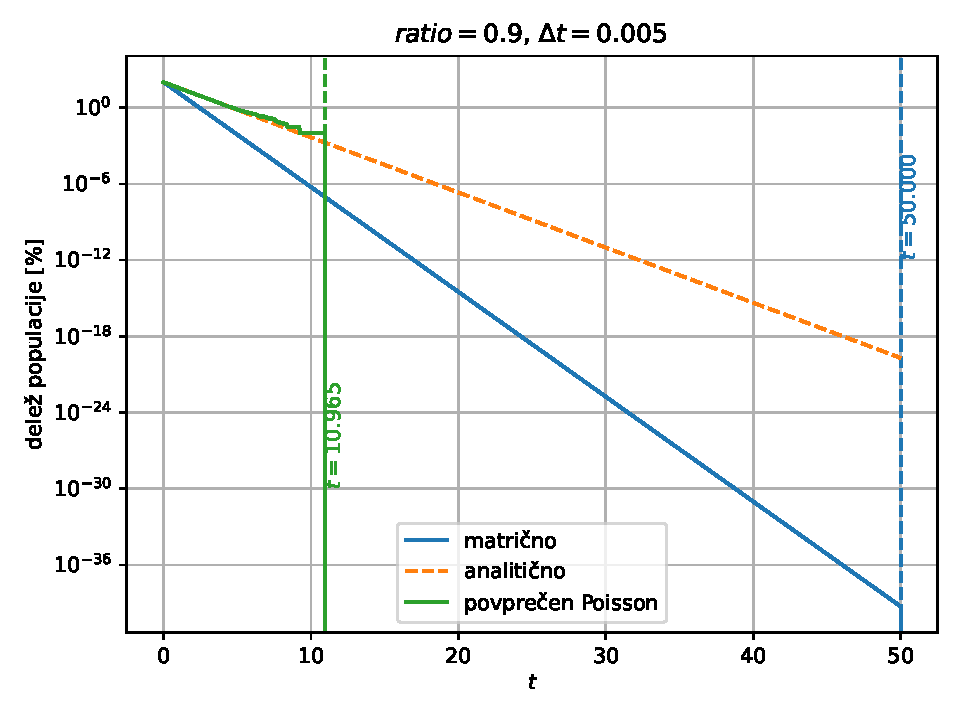
\includegraphics[width=\linewidth]{9.nal_slike/2/primerjava_ratio0.9.pdf}
        \caption{ratio = 0,9}
    \end{subfigure}
    \caption{Primerjava s Poissonsko metodo, povprečjom 100 ponovitev}
\end{figure}

\section{Model zajci - lisice}

Model Lotka-Volterra za populaciji zajcev in lisic se glasi:
\begin{align}
    \dot z &= 5\,\alpha\,z - 4\,\alpha\,z - \frac{\alpha}{L_0}\,z\,l \\ \nonumber
    \dot l &= 4\,\beta\,l - 5\,\beta\,l +\frac{\beta}{Z_0}\,z\,l
\end{align}
kjer sta $\alpha$ in $\beta$ prosta parametera za skaliranje, $Z_0, L_0$ pa začetni populaciji zajcev in lisic, ki sta v navodilih podani v ravnovesnem stanju: $Z_0=200$ in $L_0=50$.

Določeno je tudi razmerje rodnost/smrtnost zajcev 5/4 in obratno za lisice, kar je že zajeto v enačbah.

Z uporabo Poissonsko porazdeljenih števil se sistem diskretno popiše:
\begin{align}
   Z_{i+1} = Z_i + \mathcal{P}(5\,\alpha\,Z_i\,\Delta t) -\mathcal{P}(4\,\alpha\,Z_i\,\Delta t) - \mathcal{P}(\frac{\alpha}{L_0}\,Z_i\,\Delta t) \\\nonumber
   L_{i+1} = L_i + \mathcal{P}(4\,\beta\,L_i\,\Delta t) -\mathcal{P}(5\,\beta\,L_i\,\Delta t) - \mathcal{P}(\frac{\beta}{Z_0}\,L_i\,\Delta t)
\end{align}

Zaradi naključnosti ne dobimo takop lepih ciklov kot v \textit{4.nalogi}, saj ena populacija dokaj hitro izumre, zato bom podrobneje analiziral, katera prej izumre in kdaj! 

Presenetljivo, manjši časovni korak še poslabša zadevo, saj se izvede še manj ciklov. Vseeno pa cikli lisic lepo sledijo populaciji zajcev.

Iz sledečih slik ugotovim, da lisice in zajci izumrejo podobno poosto, kar NI razvidno tudi iz enačb, iz katerih gre očitno sklepati, da so lisice bolj delikatne živali od zajcev, saj imajo manjše razmerje rodnost/smrtnost.

\begin{figure}[H]
    \centering
    \begin{subfigure}{0.49\textwidth}
        \centering
        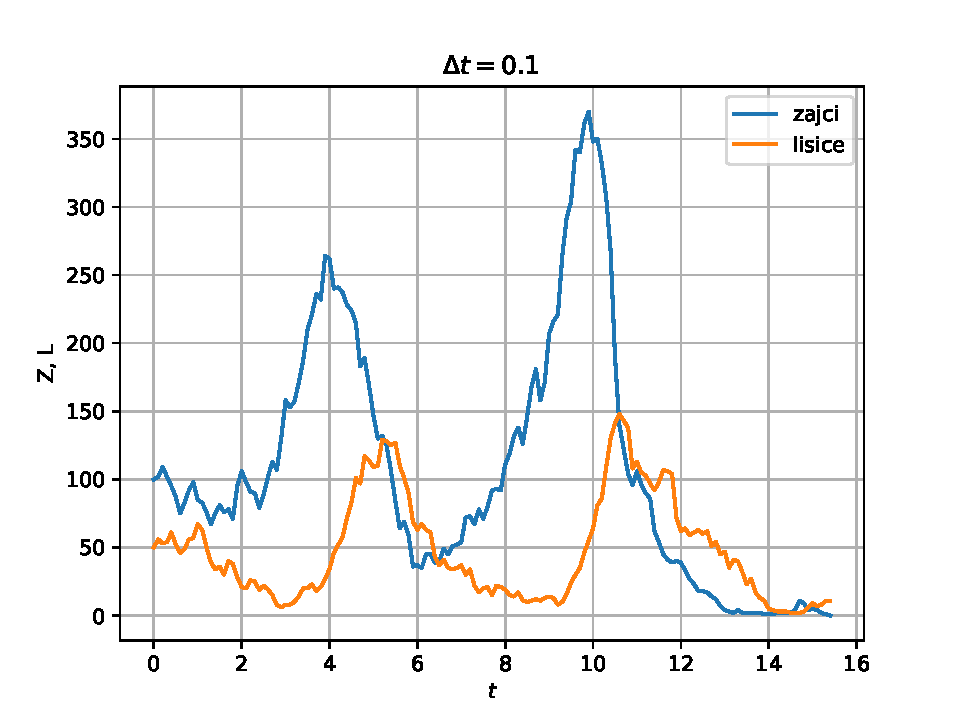
\includegraphics[width=\linewidth]{9.nal_slike/3/Z_L_dt0.1.pdf}
    \end{subfigure}
    \begin{subfigure}{0.49\textwidth}
            \centering
        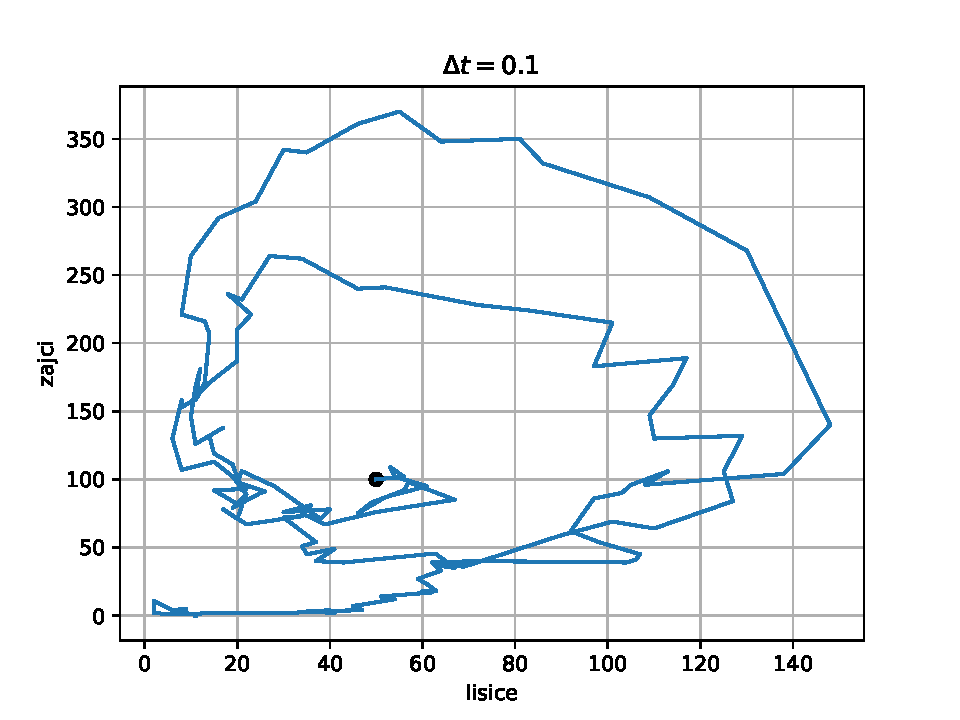
\includegraphics[width=\linewidth]{9.nal_slike/3/T_L_fazni_dt0.1.pdf}
    \end{subfigure}
    \caption{Fazni diagram in potek populacij zajcev in lisic, $\Delta t =0.1$, izumrejo zajci}
\end{figure}

\begin{figure}[ht]
    \centering
    \begin{subfigure}{0.49\textwidth}
        \centering
        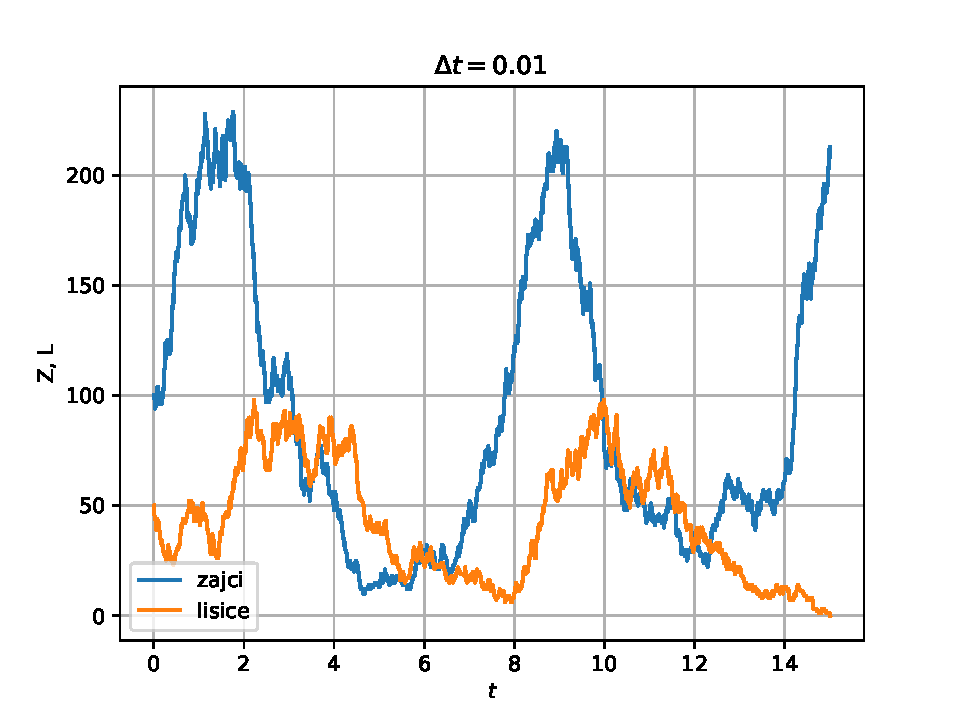
\includegraphics[width=\linewidth]{9.nal_slike/3/Z_L_dt0.01.pdf}
    \end{subfigure}
    \begin{subfigure}{0.49\textwidth}
            \centering
        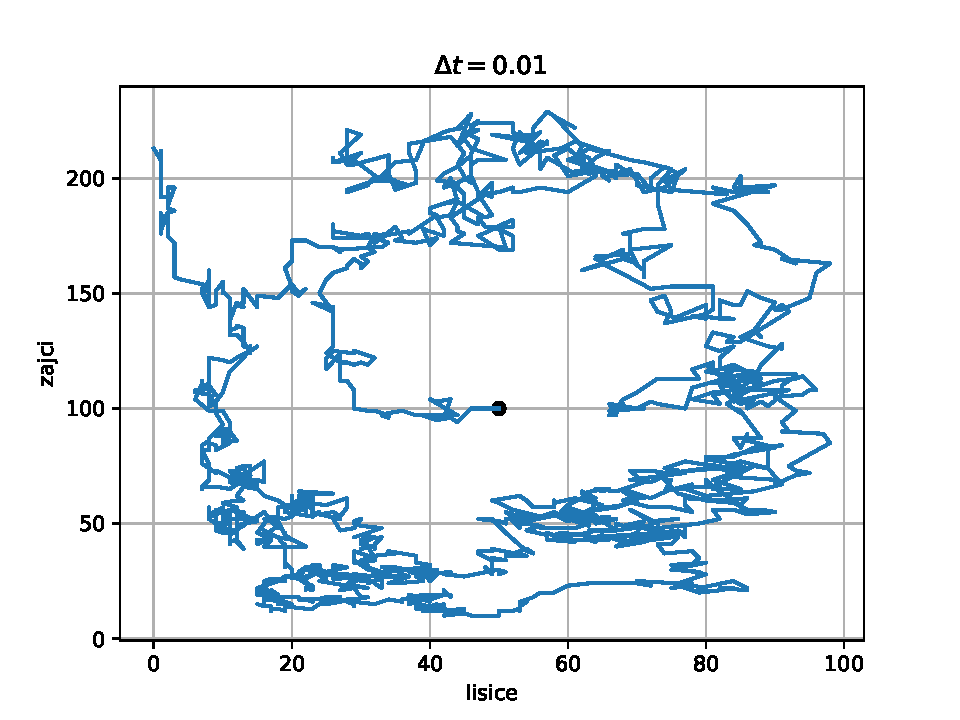
\includegraphics[width=\linewidth]{9.nal_slike/3/T_L_fazni_dt0.01.pdf}
    \end{subfigure}
    \caption{Fazni diagram in potek populacij zajcev in lisic, $\Delta t =0.01$, izumrejo lisice}
\end{figure}

\begin{figure}[ht]
    \centering
    \begin{subfigure}{0.49\textwidth}
        \centering
        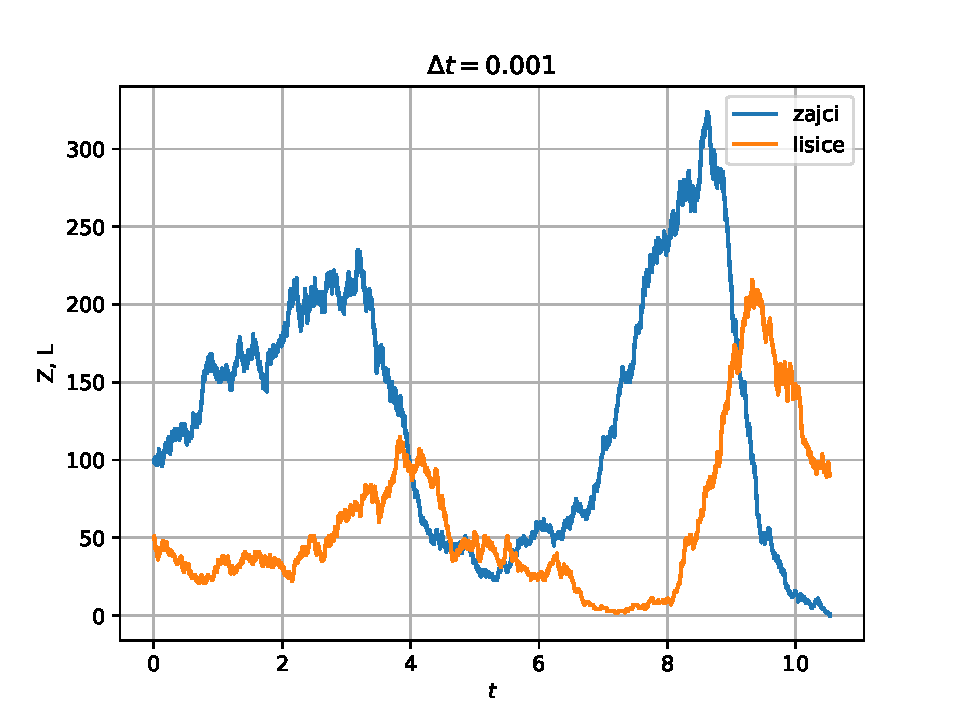
\includegraphics[width=\linewidth]{9.nal_slike/3/Z_L_dt0.001.pdf}
    \end{subfigure}
    \begin{subfigure}{0.49\textwidth}
            \centering
        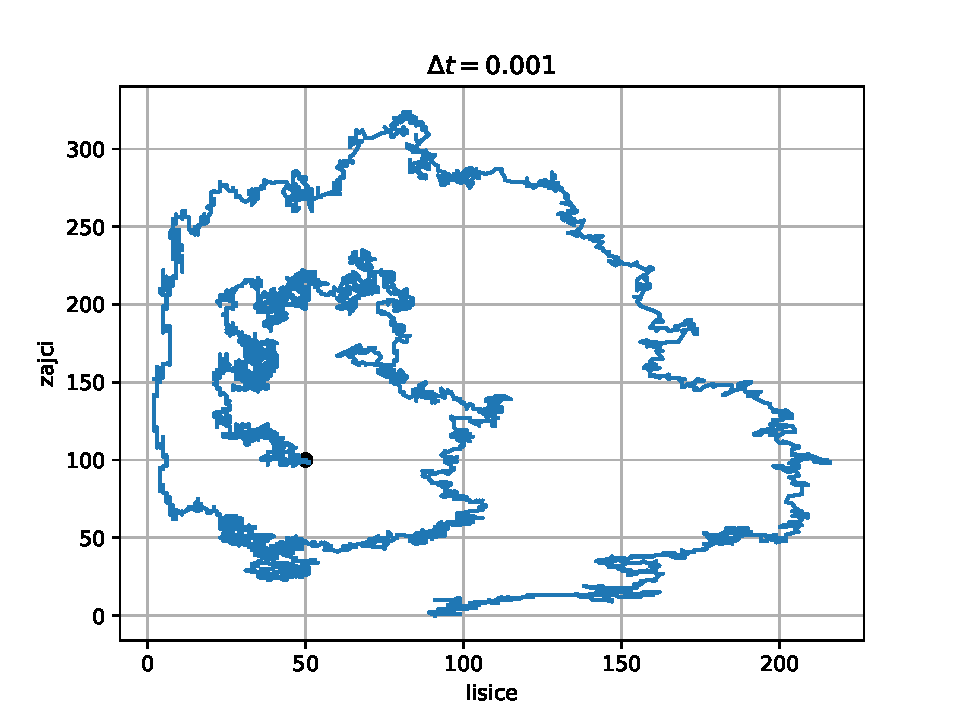
\includegraphics[width=\linewidth]{9.nal_slike/3/T_L_fazni_dt0.001.pdf}
    \end{subfigure}
    \caption{Fazni diagram in potek populacij zajcev in lisic, $\Delta t =0.001$, izumrejo zajci}
\end{figure}

\begin{figure}[H]
    \centering
    \begin{subfigure}{0.49\textwidth}
        \centering
        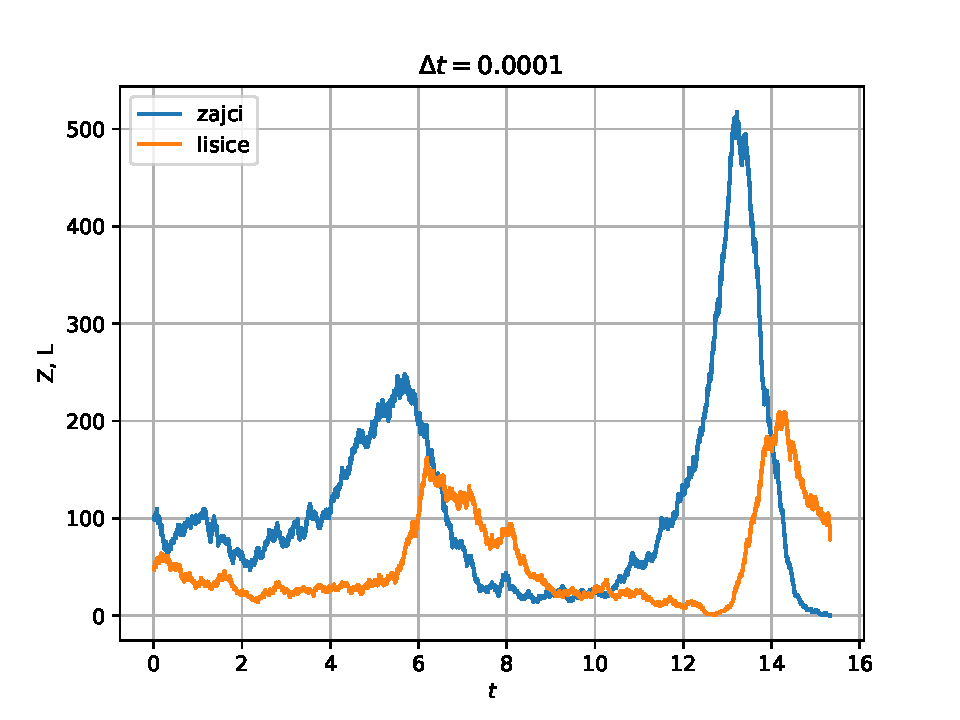
\includegraphics[width=\linewidth]{9.nal_slike/3/Z_L_dt0.0001.pdf}
    \end{subfigure}
    \begin{subfigure}{0.49\textwidth}
            \centering
        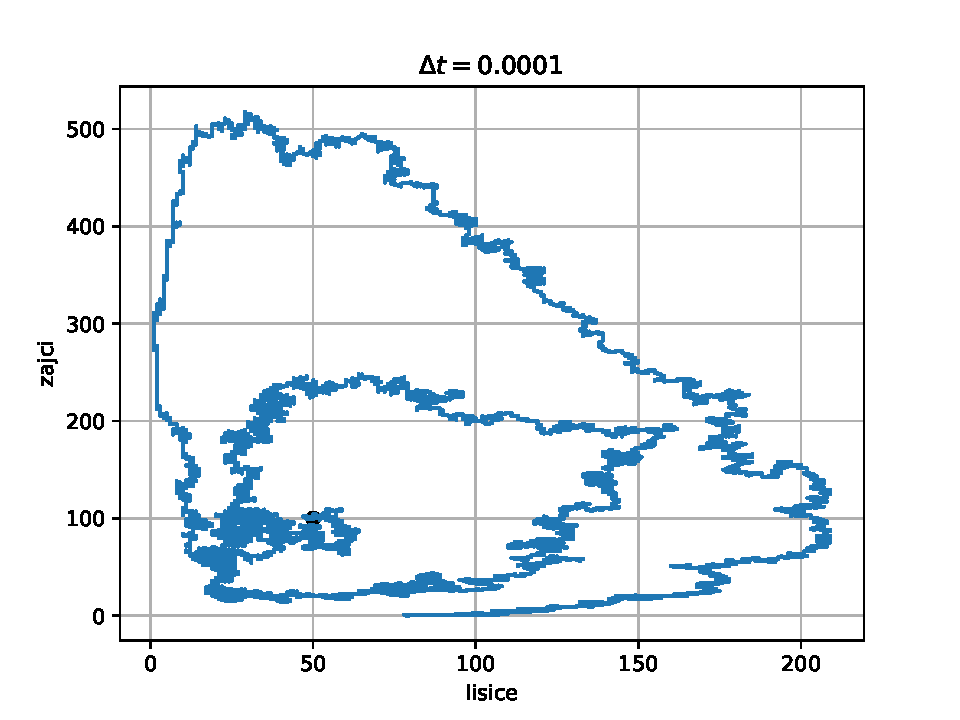
\includegraphics[width=\linewidth]{9.nal_slike/3/T_L_fazni_dt0.0001.pdf}
    \end{subfigure}
    \caption{Fazni diagram in potek populacij zajcev in lisic, $\Delta t =0.0001$, izumrejo zajci}
\end{figure}

Izvedel sem še analizo, katera vrsta izumre, na tak način, da sem upošteval večkrat izumrto vrsto v 20 ponovitvah. Kjer je nedoločeno, je število izumrtij ravno enako. V tem primeru se rezultat z manjšanjem $\Delta t$ izboljša, vendar izgleda, kot da vedno pogosteje izumirajo zajci! Da bi analiziral še odvisnost od začetnih pogojev in razmerja rodnost/smrtnost se model izkaže za preveč naključnega! To je bolj smiselno analizirati s časovno integracijo diferencialnih enačb.

\begin{figure}[H]
    \centering
    \begin{subfigure}{0.49\textwidth}
        \centering
        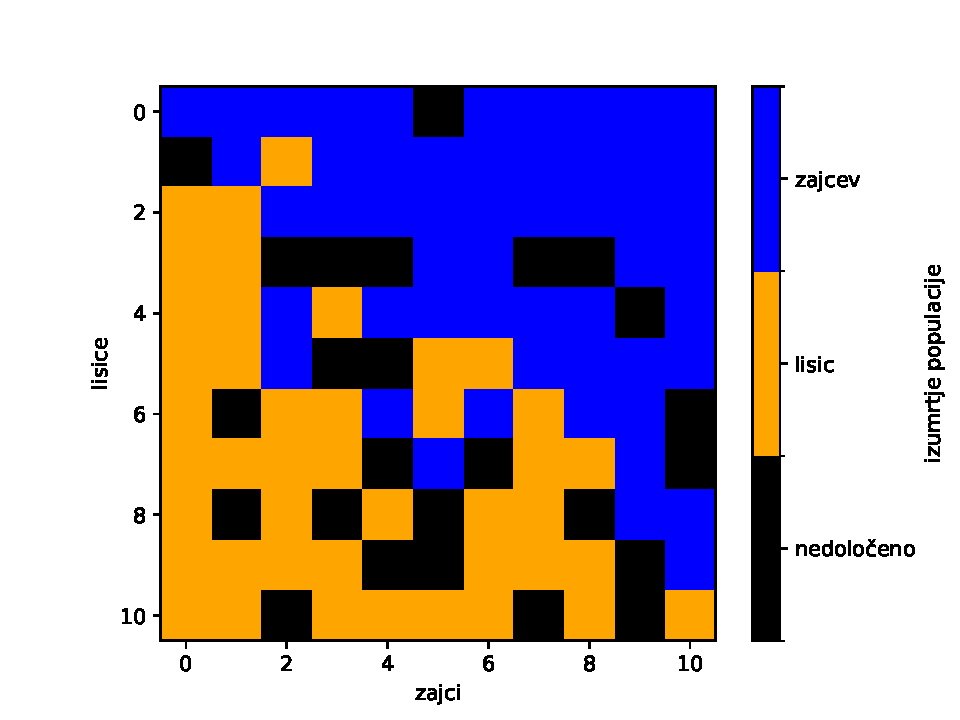
\includegraphics[width=\linewidth]{9.nal_slike/3/Z_L_colormap_dt0.1.pdf}
        \caption{$\Delta t = 0,1$}
    \end{subfigure}
    \begin{subfigure}{0.49\textwidth}
            \centering
        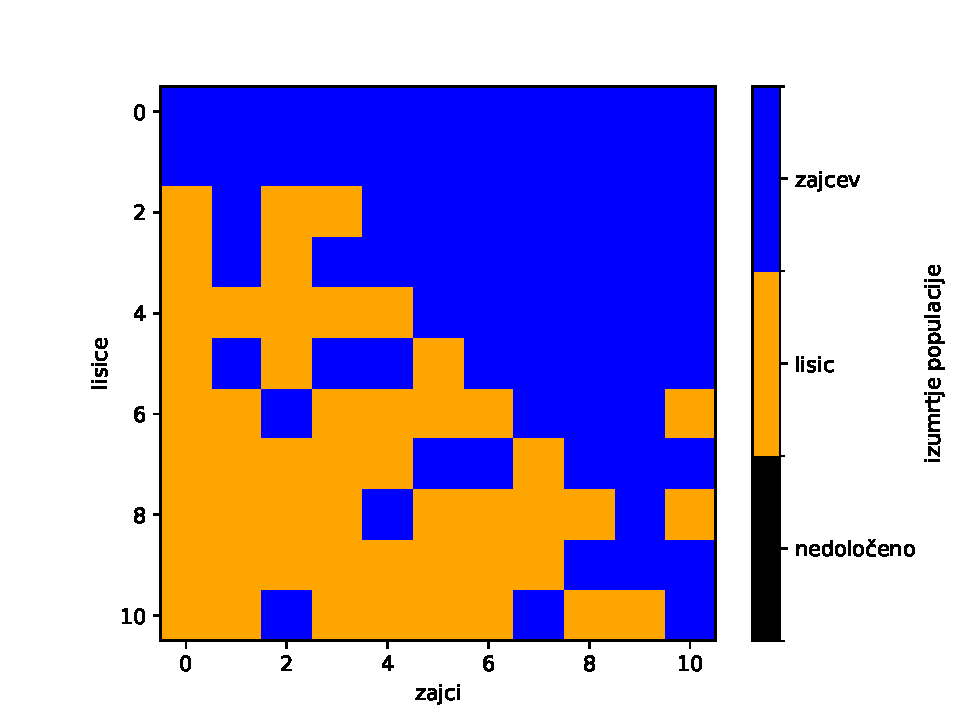
\includegraphics[width=\linewidth]{9.nal_slike/3/Z_L_colormap_dt0.01.pdf}
        \caption{$\Delta t = 0,01$}
    \end{subfigure}
    \begin{subfigure}{0.49\textwidth}
        \centering
        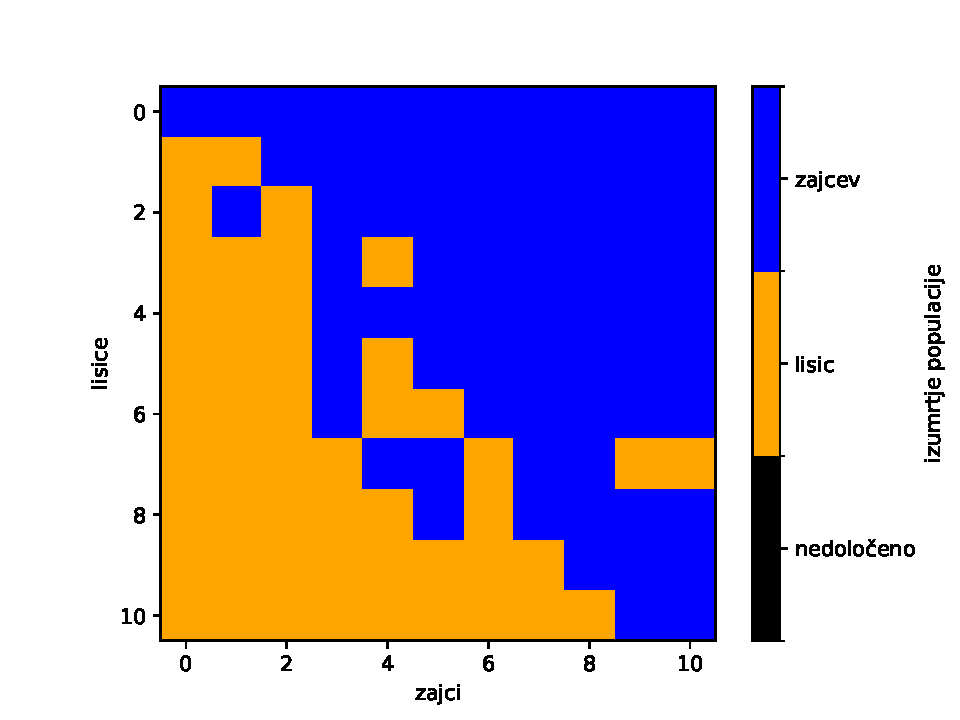
\includegraphics[width=\linewidth]{9.nal_slike/3/Z_L_colormap_dt0.001.pdf}
        \caption{$\Delta t = 0,001$}
    \end{subfigure}
    \caption{Prikaz največkrat izumrte živali v 20 ponovitvah, $Z_0=100$, $L_0=50$}
\end{figure}
%spreminjanje ZP - (pre)več parametrov!

Sledi še prikaz porazdelitve časov izumrtja. Kot to sem upošteval tako zajce, kot lisice. Porazdelitev je podobna oni iz prejšnje naloge.

\begin{figure}[ht]
    \centering
    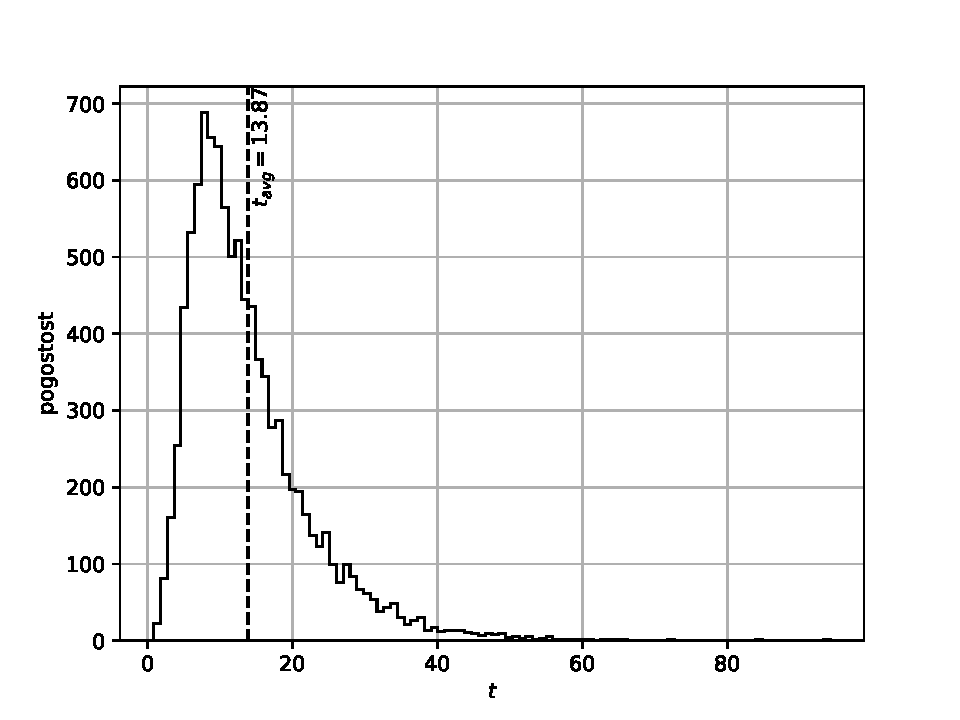
\includegraphics[width=0.7\textwidth]{9.nal_slike/3/izumrtje_Z_L.pdf}
    \caption{Histogram porazdelitve časov izumrtja za 10 000 ponovitev}
\end{figure}

\section{Model epidemije}

Na spodji sliki je prikazan preprost model epidemije, za katerega velja spodnji sistem diferencialnih enačb za 3 pod-populacije oseb, bolne dovzetne in imune. Levo je prikazana osnovna oblika, desno pa brezdimenzijska.

\begin{align}\label{eqn:4}
    \dot D &= -\alpha \, D \, B & \dot D &= -R_r \, D \, B + I_r \, I\\ \nonumber
    \dot B &= \alpha \, D \, B - \beta \, B & \dot B &= R_r \, D \, B -B \\ \nonumber
    \dot I &= \beta \, B - \gamma \, I & \dot I &= B - I_r \, I 
\end{align}
kjer je $R_r=\alpha/\beta$ reprodukcijsko število, ki opisuje, kako hitro se širi okužba in $I_r=\gamma/\beta$ razmerje imunosti in opisuje, kako hitro prehajajo osebki iz populacije imunih v dovzetene. stohastčen model podajajo spodnje enačbe, kjer je $N_0$ začetna velikost populacije, ki je konstantna!

\begin{align}\label{eqn:4}
    D &= D - \mathcal{P}(R_r\,D\,B\,\Delta t/N_0) + \mathcal{P}(I_r\,I\,\Delta t) \\ \nonumber
    B &= B + \mathcal{P}(R_r\,D\,B\,\Delta t/N_0) - \mathcal{P}(B\,\Delta t) \\ \nonumber
    I &= I + \mathcal{P}(B\,\Delta t) - \mathcal{P}(I_r\,I\,\Delta t)
\end{align}

Model lahko nadgradimo z upoštevnjem rojstev in smrti, s čimer pridobimo nova parametra $M_r$ in $N_r$. V tem primeru populacija raste, saj smrti upoštevamo kot pod-populacijo.
\begin{align}\label{eqn:6}
    \dot D &= -\alpha \, D \, B + \varepsilon \, (D+I) & \dot D &= -R_r \, D \, B + I_r \, I + N_r \, (D+I)\\ \nonumber
    \dot B &= \alpha \, D \, B - \beta \, B - \delta \, B & \dot B &= R_r \, D \, B - B - M_r \, B \\ \nonumber
    \dot I &= \beta \, B - \gamma \, I & \dot I &= B - I_r \, I \\ \nonumber
    \dot M &= \delta B & \dot M &= M_r \, B
\end{align}

Na spodnji sliki se vidi, da dobimo primerljive rezultate s stohastičnim modelom, kot z numerično integracijo v času, prav tako pa se potek spremeni, ko dodamo smrti in rojstva, kjer se vrh zniža in zakasni, epidemija pa težje
izgine.

\begin{figure}[ht]
    \centering
    \begin{subfigure}{\textwidth}
        \centering
        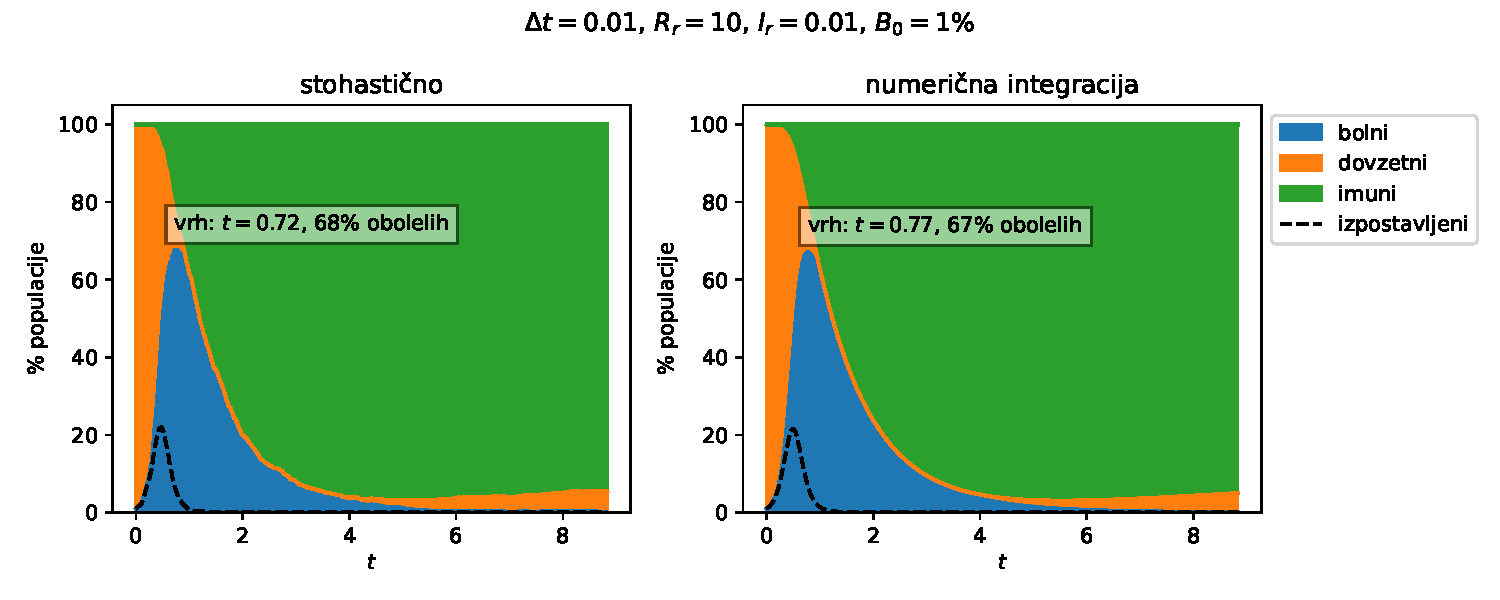
\includegraphics[width=\linewidth]{9.nal_slike/4/potek_ozdravitev.pdf}
        \caption{reprodukcijsko število $R_r=10$, razmerje imunosti $I_r=0,01$}
    \end{subfigure}
    \begin{subfigure}{\textwidth}
            \centering
        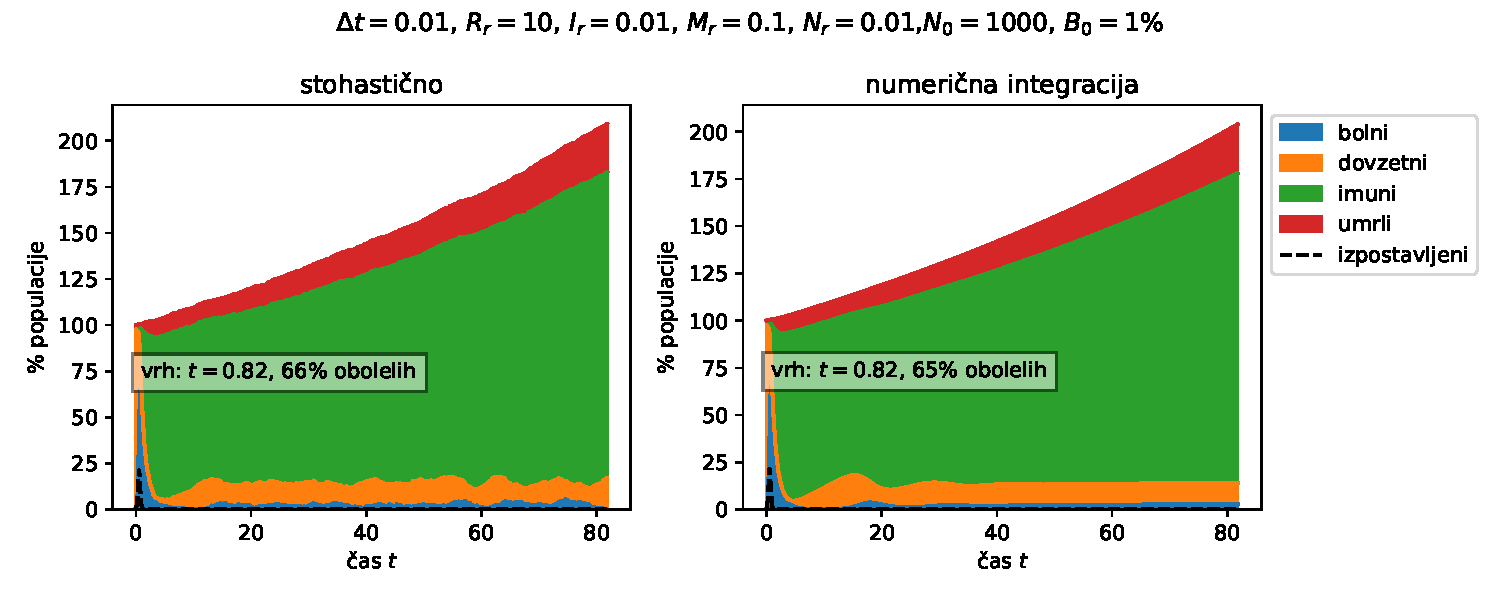
\includegraphics[width=\linewidth]{9.nal_slike/4/potek_smrti_rojstva.pdf}
        \caption{dodane smrti $M_r$, rojstva $N_r$}
    \end{subfigure}
    \caption{Potek deležev, če je na začetnu okužen 1\% populacije}
\end{figure}

Preizkusil sem tudi, kako parametra vpivata na vrh epidemije, kjer sem upošteval povprečno višino vrha 20 ponovitev in opazij, da nanj vpliva le razm. imunosti.
\begin{figure}[ht]
    \centering
    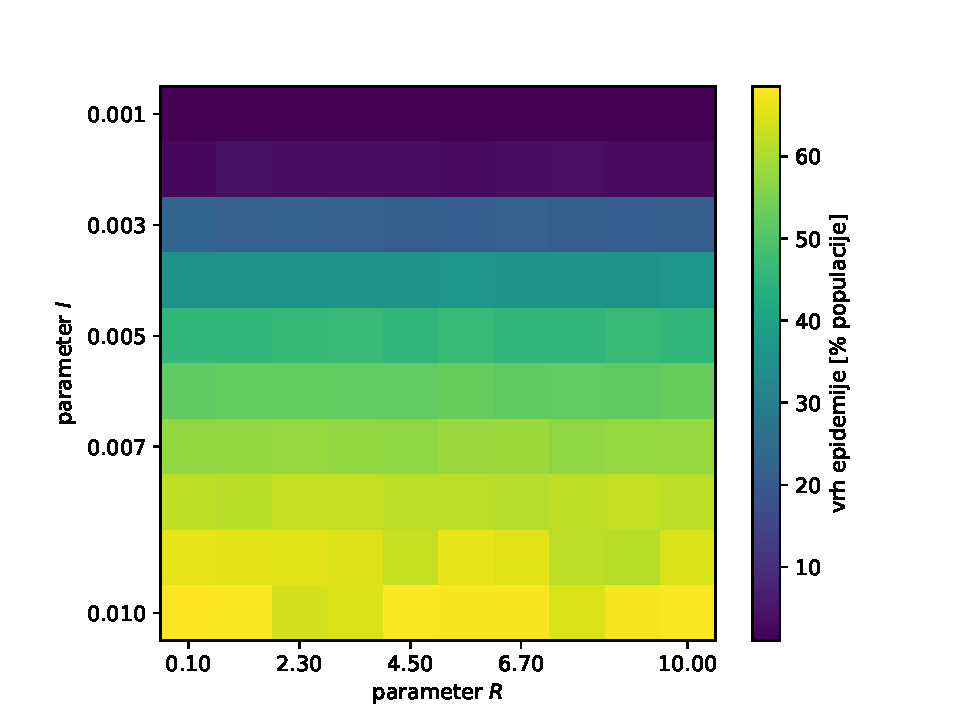
\includegraphics[width=0.7\linewidth]{9.nal_slike/4/vrh_epidemija_cmap.pdf}
    \caption{Višina vrha bolnih je neodvisna od reprodukcijekega števila $R_r$!}
\end{figure}

Podobno velja za čas nastopa vrha bolnih in čas izumrtja bolezni, le da je ta tokrat odvisna od reprodukcijskega števila in ima prevej velik raztros pri manjših vrednostih, pri večjih pa konvergira blizu vrednosti t=8.

Pri spreminjanju velikosti populacije, v območju (100, 1000), se porazdelitev premika v desno, torej k daljšim časom. Za vse spodnje simulacije so bili uporabljeni sledeči parametri, če ni na sliki prikazano drugače: $R_r=5$, $I_r=0,001$ in $N_0=1000$.

\begin{figure}[ht]
    \centering
    \begin{subfigure}{0.49\textwidth}
        \centering
        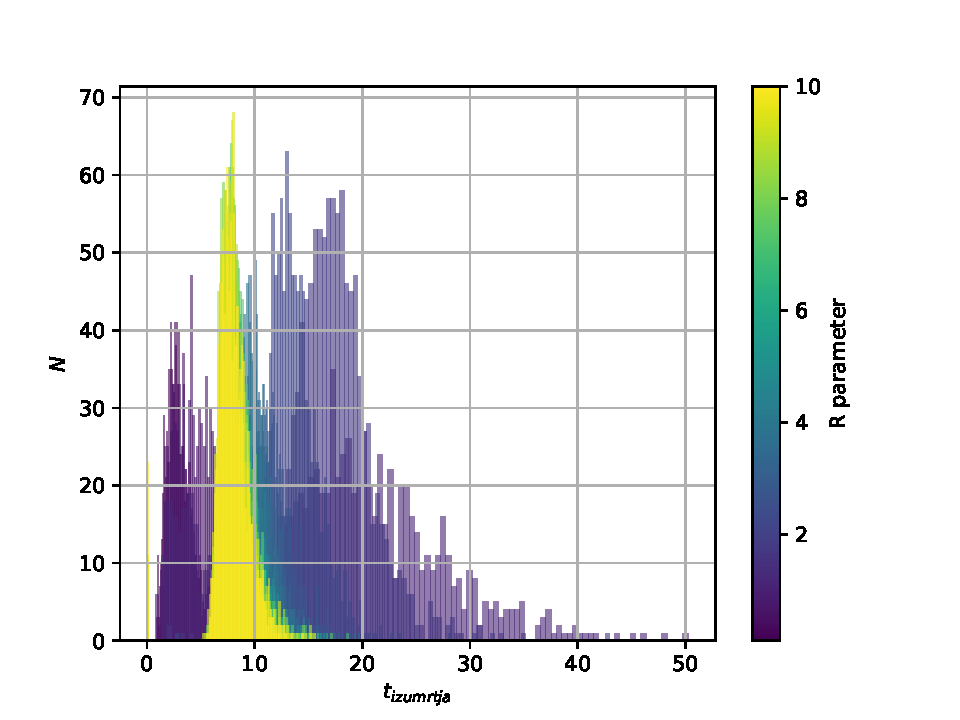
\includegraphics[width=\linewidth]{9.nal_slike/4/hist_R.pdf}
        \caption{glede na $R_r$}
    \end{subfigure}
    \begin{subfigure}{0.49\textwidth}
        \centering
        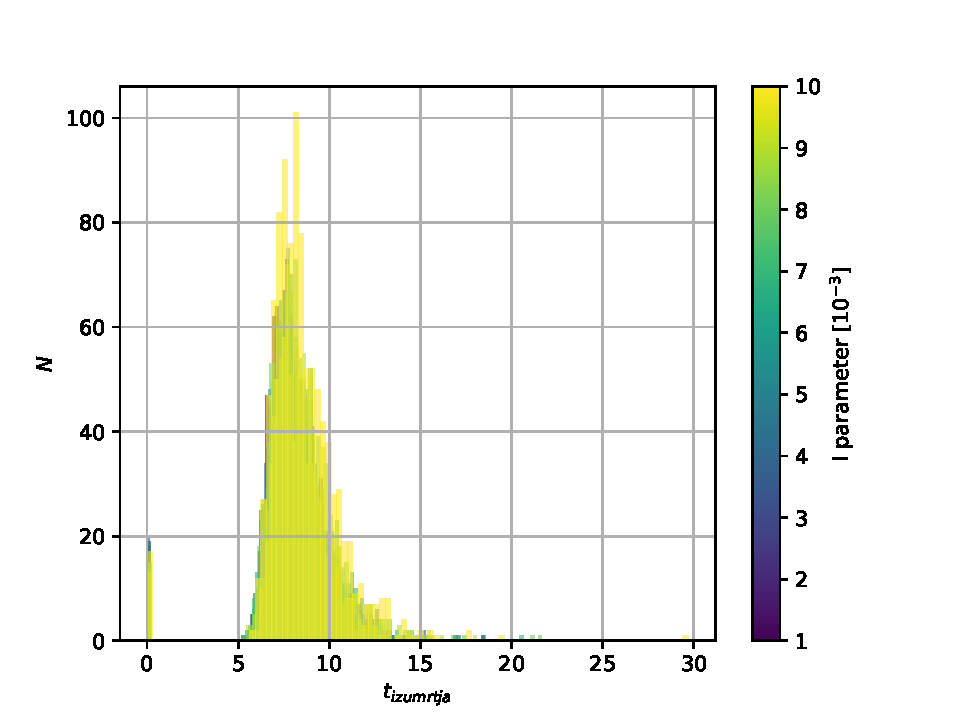
\includegraphics[width=\linewidth]{9.nal_slike/4/hist_I.pdf}
        \caption{glede na $I_r$}
    \end{subfigure}
    \begin{subfigure}{0.49\textwidth}
        \centering
        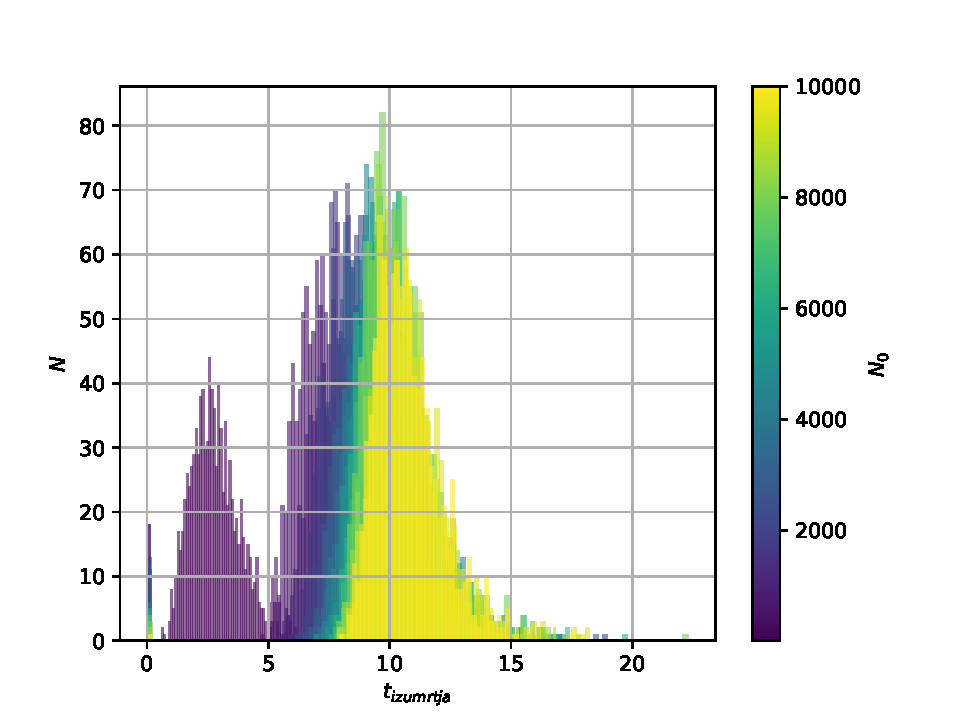
\includegraphics[width=\linewidth]{9.nal_slike/4/hist_N0.pdf}
        \caption{glede na $N_0$}
    \end{subfigure}
    \caption{Porazdelitev časov izumrtja bolezni je neodvisna od razmerja imunosti $I_r$}
\end{figure}